% Appendix A

\begin{appendices}

\addtocontents{toc}{\protect\setcounter{tocdepth}{2}}
\makeatletter
\addtocontents{toc}{%
  \begingroup
  \let\protect\l@chapter\protect\l@section
  \let\protect\l@section\protect\l@subsection
}
\makeatother

%\label{AppendixA} % For referencing this appendix elsewhere, use \ref{AppendixA}
%\counterwithin{figure}{section}
%\counterwithin{table}{section}

\newpage
.

\chapter{Attracting attention}
%\setcounter{figure}{0}
%\setcounter{table}{1}

\section{Glance count sheet}

\begin{figure}[H]
 \centering 
    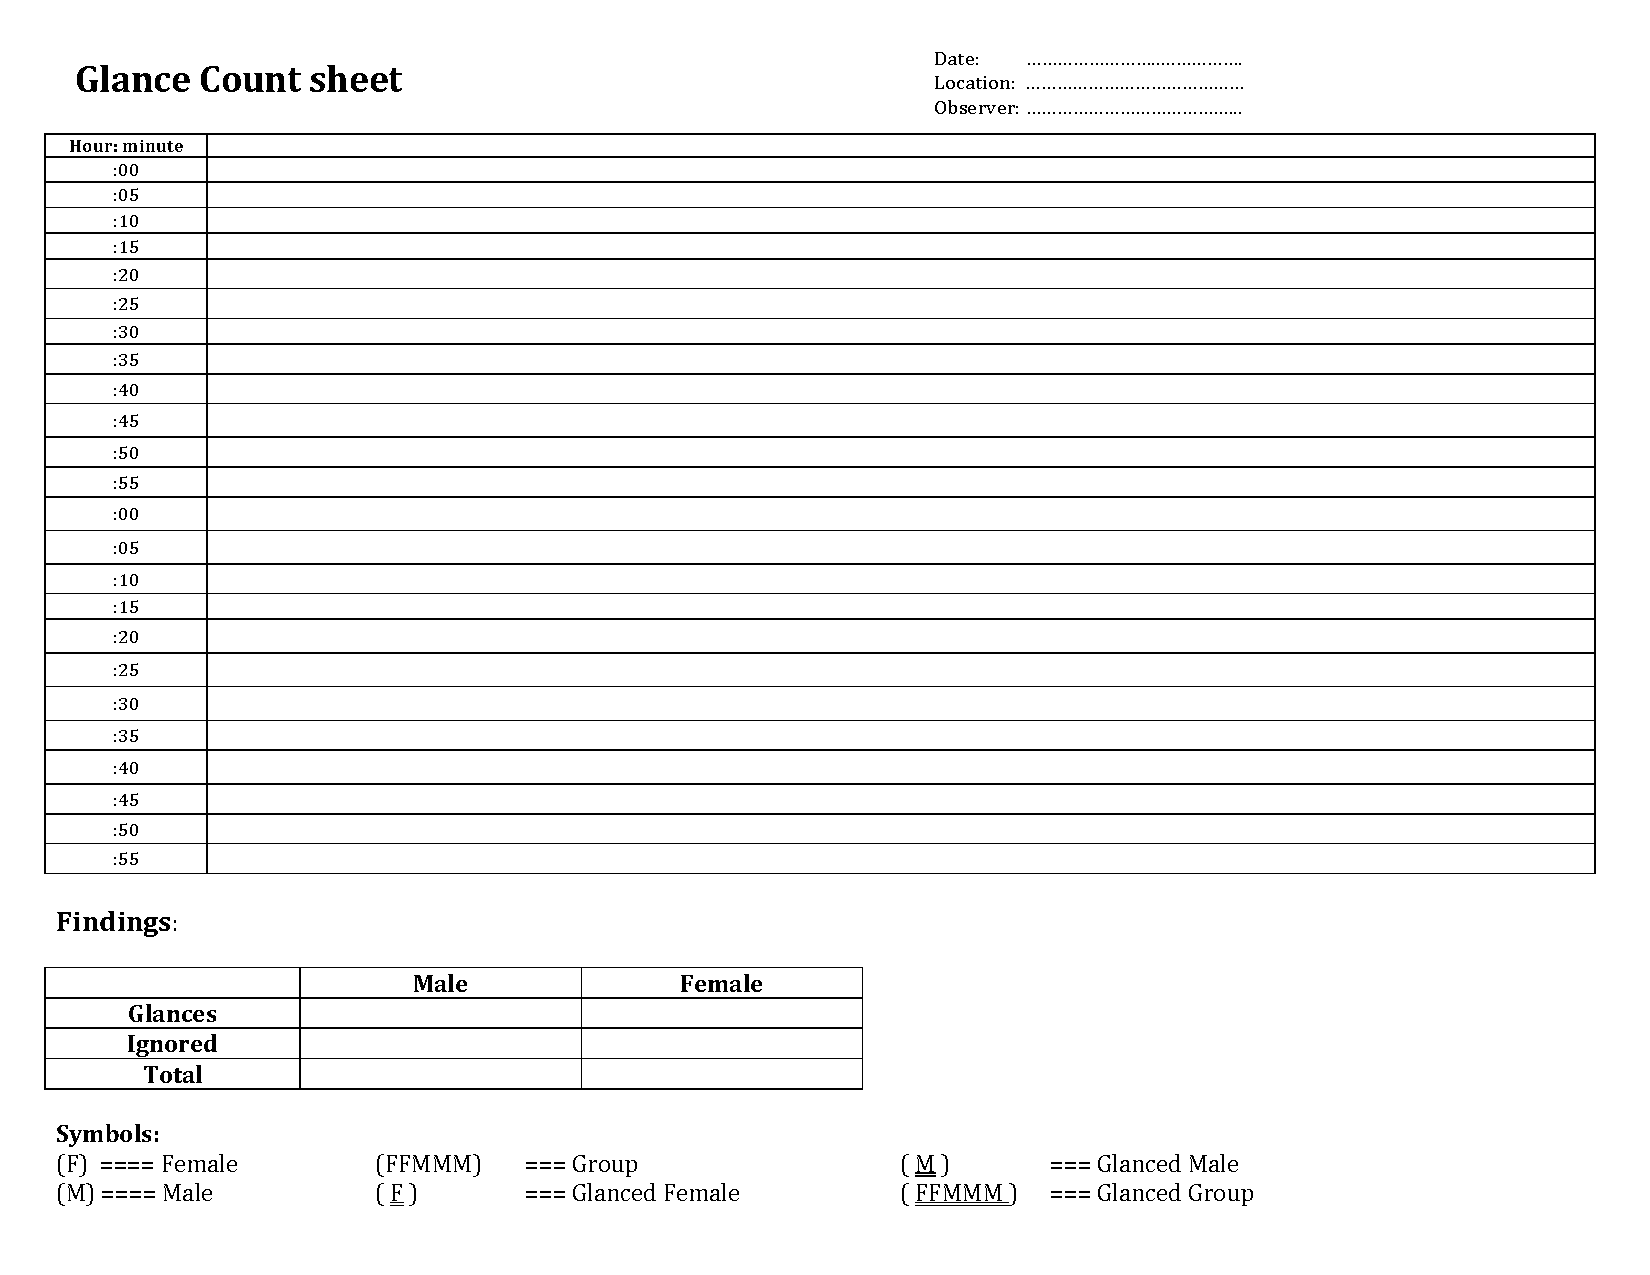
\includegraphics[width=\textwidth,height=100mm]{Appendices/3/Glance_Count_Method.pdf}
    \caption{Glance count sheet}
     \label{app:Glance_Count_Method}%
\end{figure}


\section {Interview Questionnaire}
\setcounter{table}{1}
\begin{table}[H]
\caption{Questions}
\label{app:interviewquestions}
\resizebox{\textwidth}{!}{ 
\centering
\small
\begin{tabular}{ l  l  c}
\toprule
\tabhead{No.} & \tabhead{Research Questions} \\
\midrule
1   &  Do you like advertisement on displays?          \\
2   &  Which kind of advertisement do you like?                 \\
3   &  What is that makes advertisement annoying or interested for you?   \\
4   &  What attracted you toward the screen?   \\
5   &  What do you think about this type of technique?   \\
6   &  Do yo have any other recommendations?   \\
7   &  What do you know about Interactive Advertisement?   \\
8   &  What is your expectation about interactive advertisement?   \\
\bottomrule
\end{tabular}
}
\end{table}


\section{Interview consent form}
\setcounter{figure}{2}

\begin{figure}[H]
 \centering 
    \includegraphics[width=\textwidth,height=150mm]{Appendices/3/Consent_form.pdf}
    \caption{Interview consent form}
     \label{app:concentform}%
\end{figure}

\section {Interview Color codes}

\begin{figure}[H]
 \centering 
    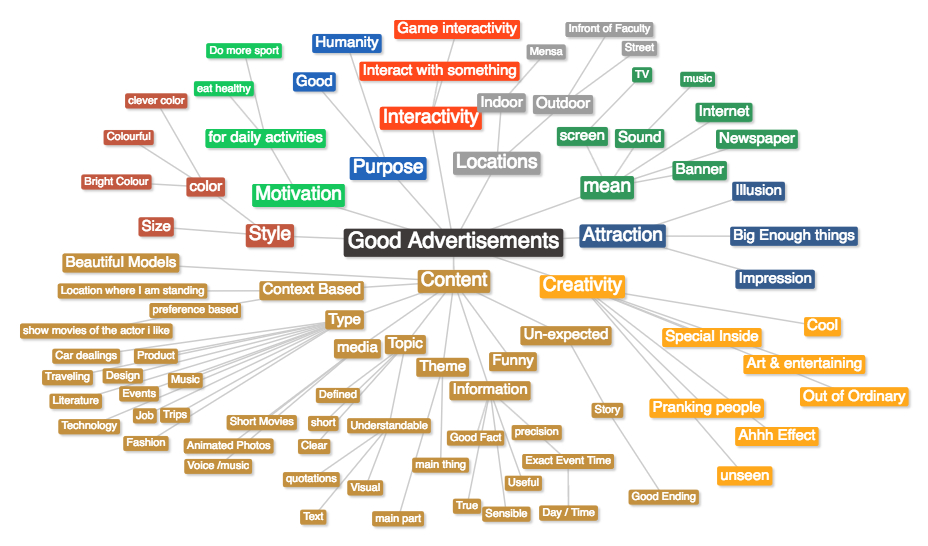
\includegraphics[width=\textwidth,height=0.4\textheight]{Appendices/3/good_ad.jpg}
    \caption{Good Advertisement}
     \label{app:goodadver}%
\end{figure}



\begin{figure}[H]
 \centering 
    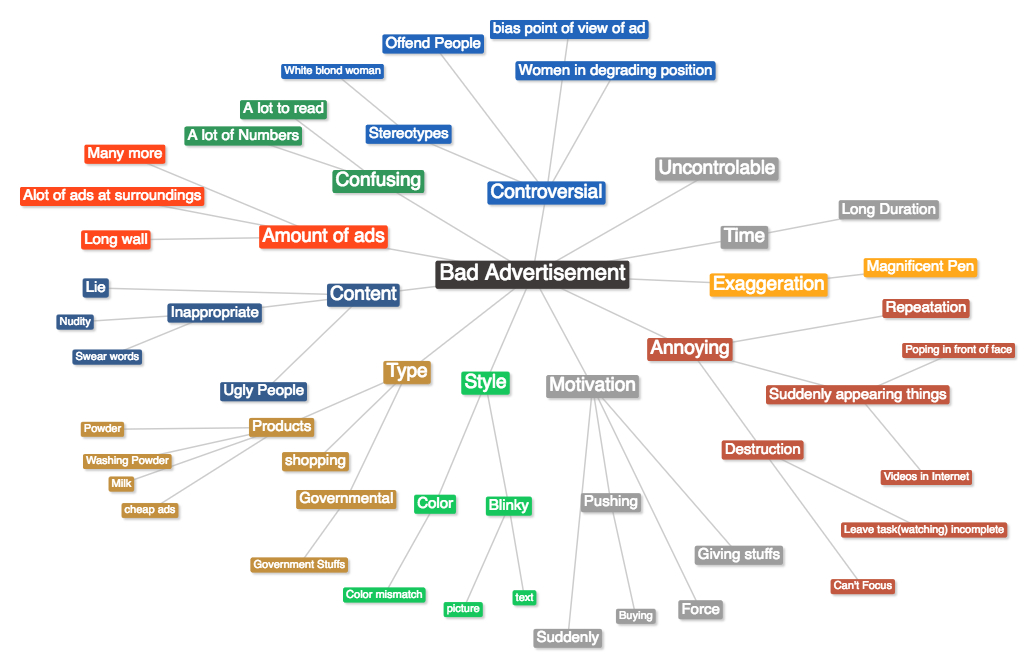
\includegraphics[width=\textwidth,height=0.45\textheight]{Appendices/3/bad_ad.jpg}
    \caption{Bad Advertisement}
     \label{app:badadver}%
\end{figure}


%\includepdf[scale=0.7,clip,trim=0cm 0cm 0cm 2cm,pages={1},pagecommand={\section{Consent Form}\subsection{part1}}]{Appendices/3/Consent_form.pdf}

\chapter{Focus Group}
% reset the figure counting

\section{First sketch}
\begin{figure}[H]
    \centering
    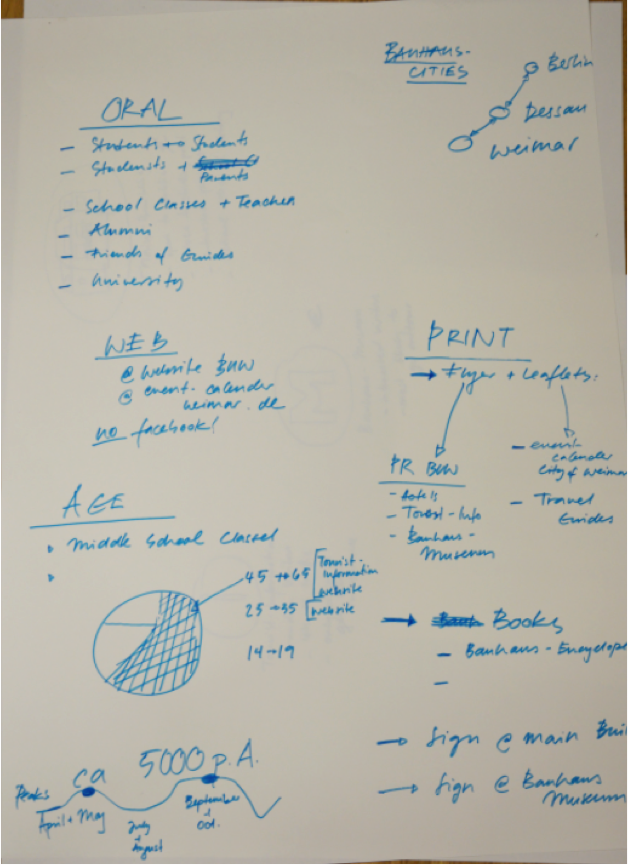
\includegraphics[width=\textwidth,height=0.8\textheight]{Appendices/4/sk1}%
    \caption{First sketch}%
    \label{app:Sk1}%
\end{figure}

\section{Second sketch}

\begin{figure}[H]
    \centering
    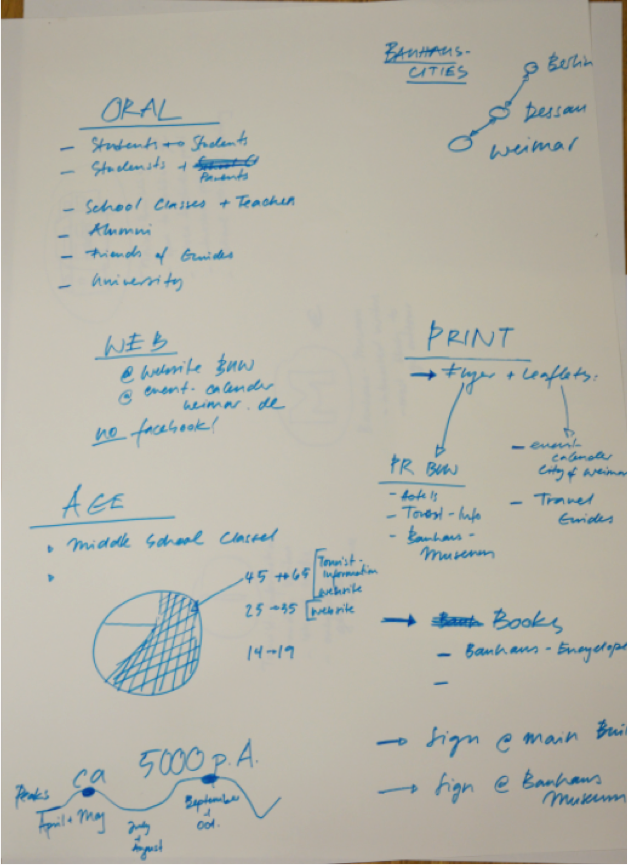
\includegraphics[width=\textwidth,height=0.8\textheight]{Appendices/4/sk2}%
    \caption{Second sketch}%
    \label{app:Sk2}%
\end{figure}


\section{Third sketch}

\begin{figure}[H]
    \centering
    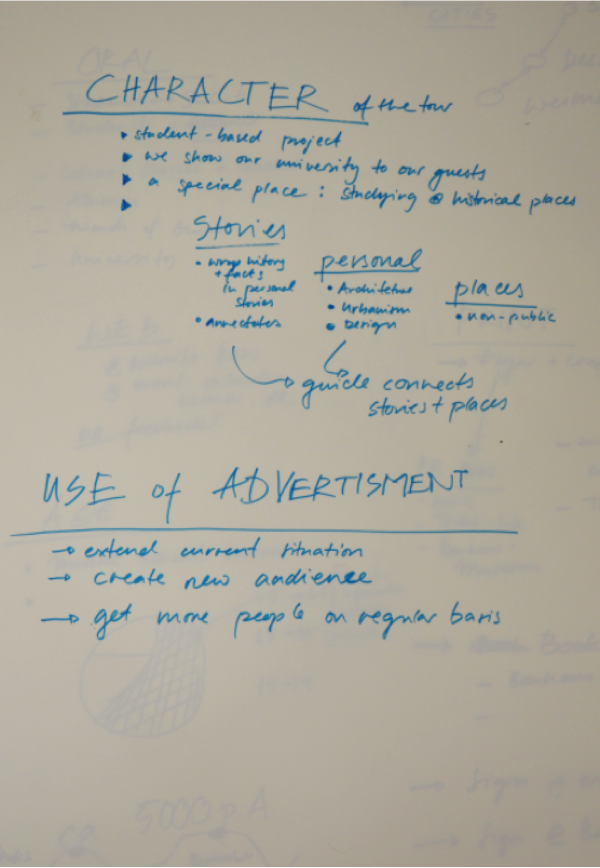
\includegraphics[width=\textwidth,height=0.8\textheight]{Appendices/4/sk3}%
    \caption{Third sketch}%
    \label{app:Sk3}%
\end{figure}


\newpage

\chapter{Low Fidelity}

\setcounter{figure}{0}
\setcounter{table}{0}

\section{Coded Interviews}
% reset the figure counting
\begin{figure}[H]
 \centering 
    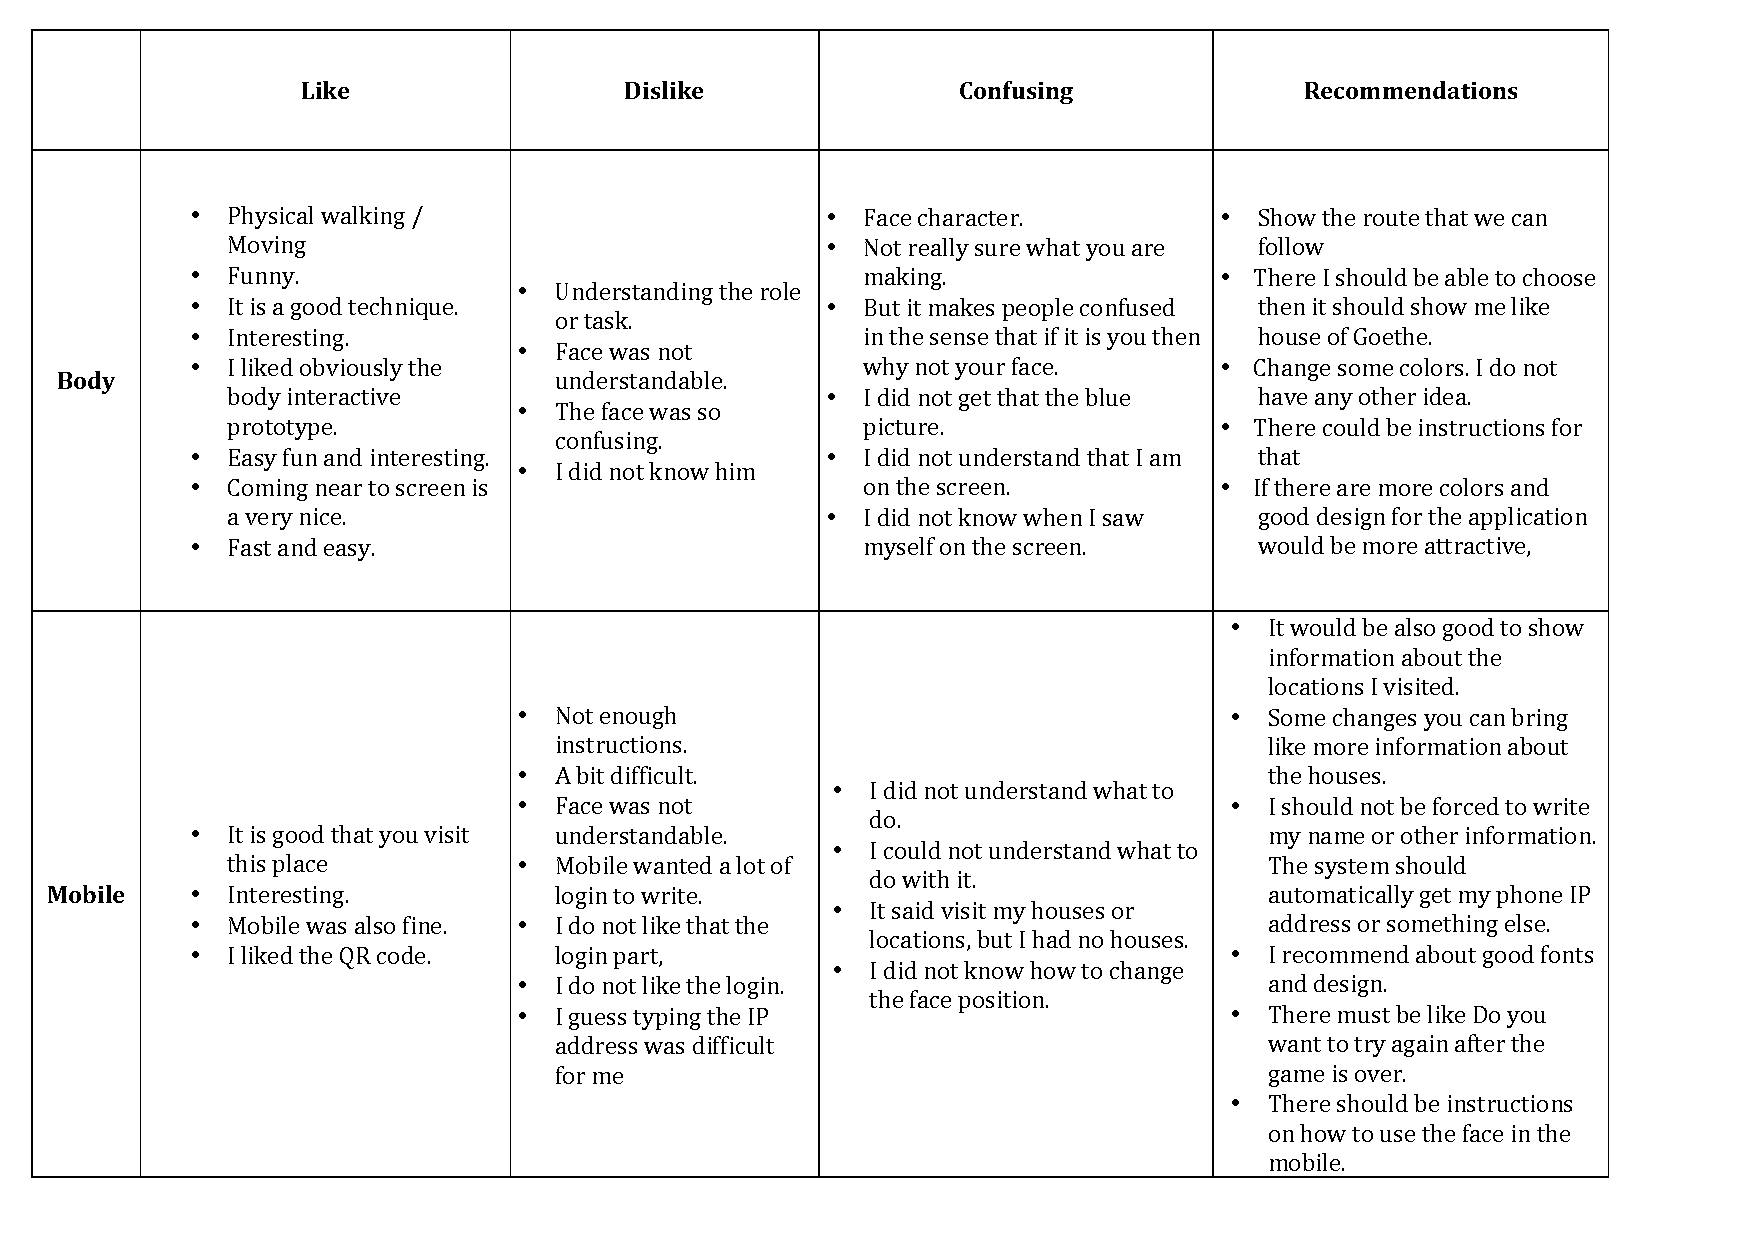
\includegraphics[width=\textwidth]{Appendices/5/Coded_Interview.pdf}
    \caption{Interview codes}
     \label{app:coded_interview}%
\end{figure}


\newpage
% Hifi- usability
\chapter{High Fidelity}

\setcounter{figure}{0}
\setcounter{table}{0}

\section{Body Interview codes}
\begin{minipage}{1.14\textwidth}
\begin{flushleft} 
\begin{figure}[H]
 \centering 
    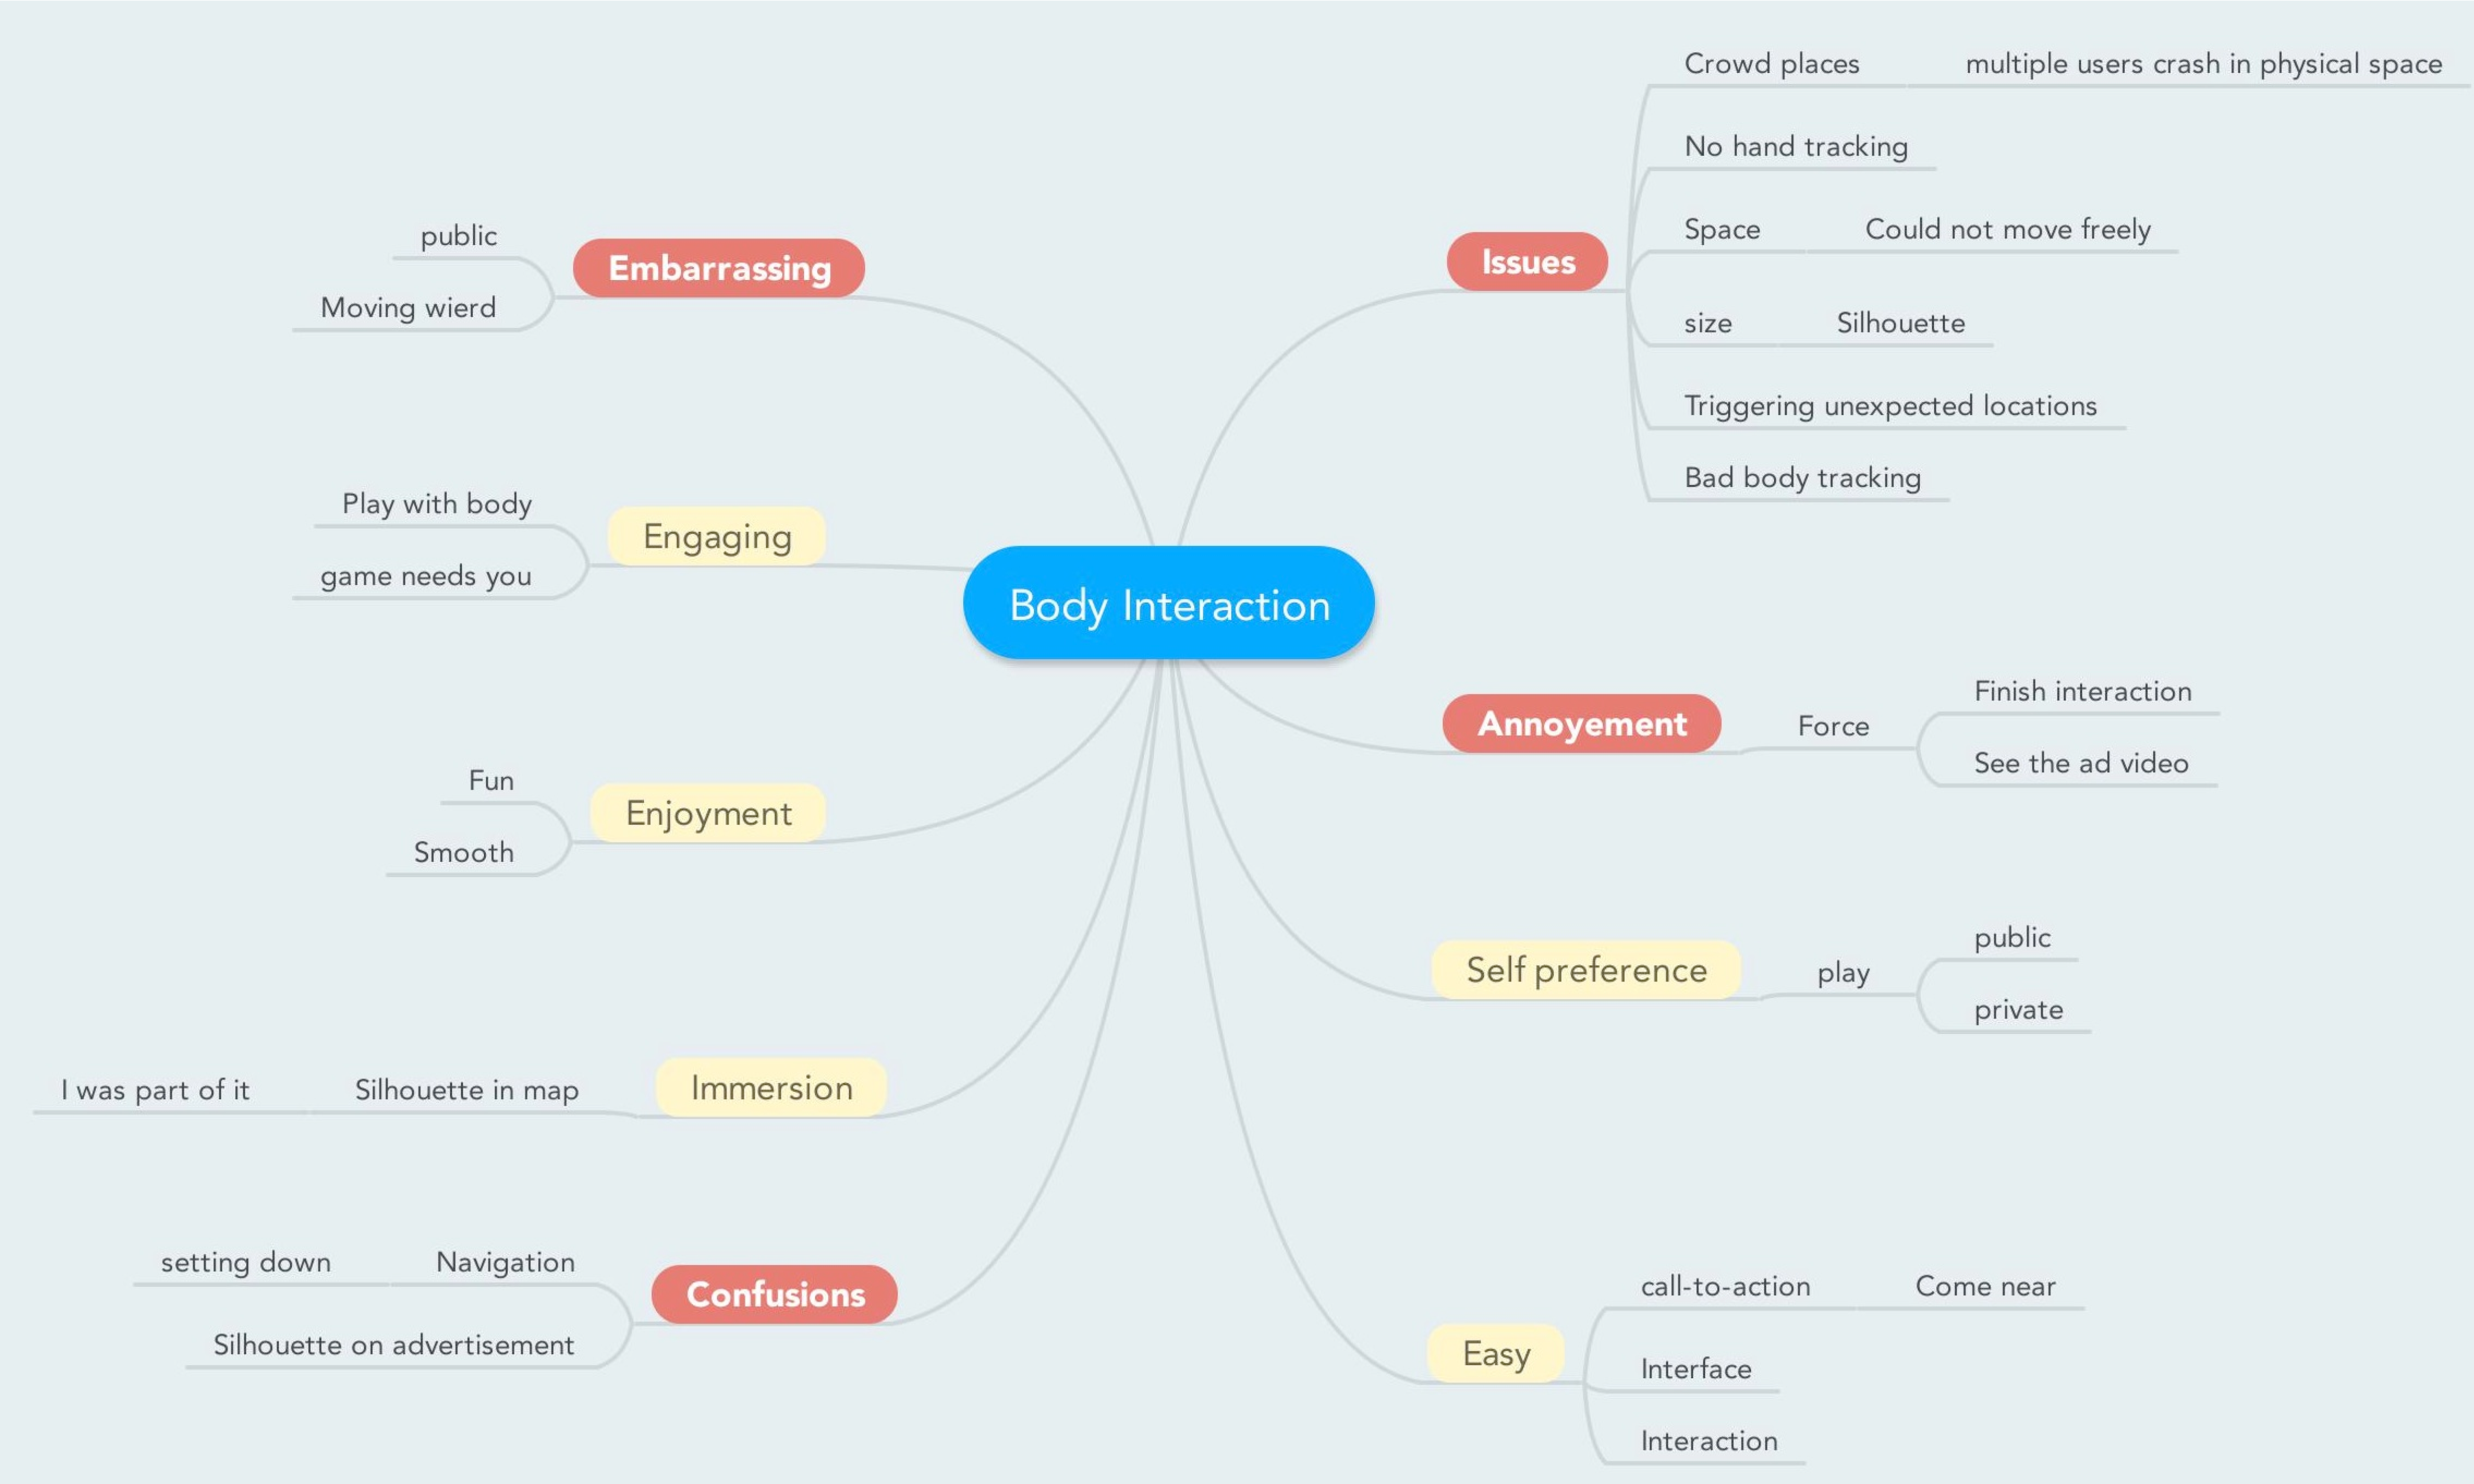
\includegraphics[width = \textwidth, height=0.8\textheight]{Appendices/6/Body_Interaction.pdf}
    \caption{Body Interview codes}
     \label{app:bodyinterviewcodes_}%
\end{figure}
\end{flushleft} 
\end{minipage}


\section{Mobile Interview codes}
\begin{minipage}{1.14\textwidth}
\begin{flushleft} 
\begin{figure}[H]
 \centering 
    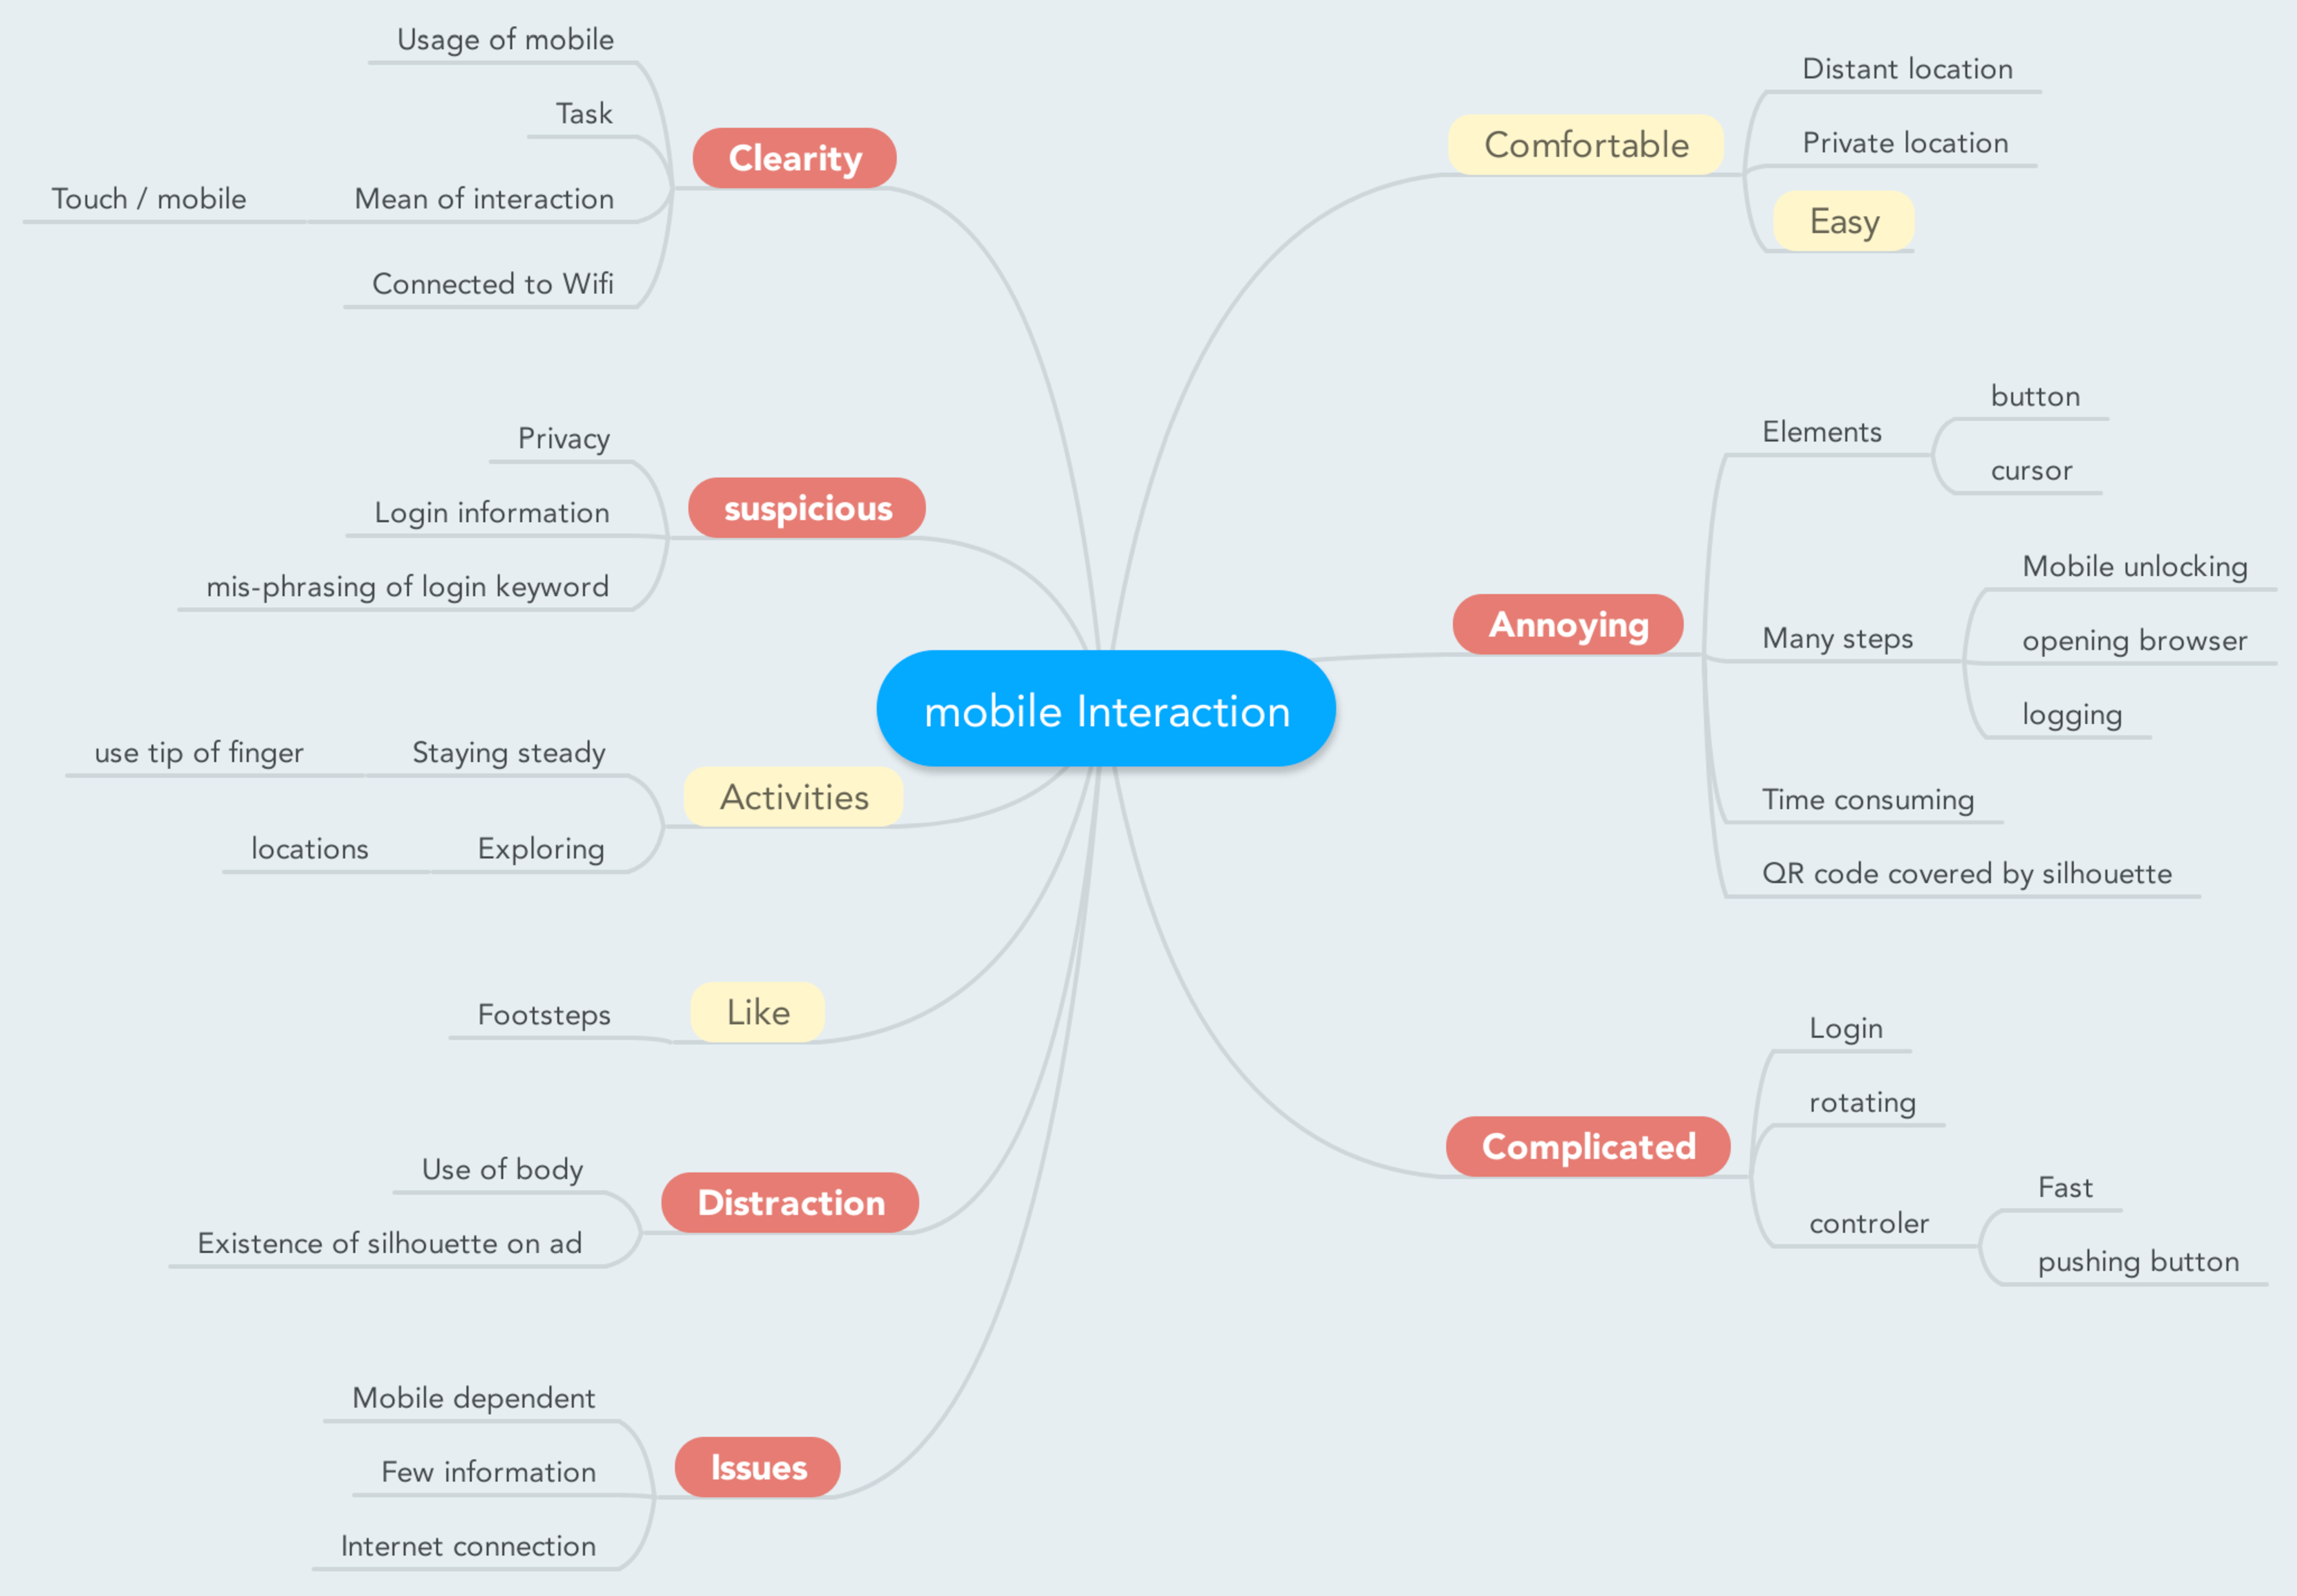
\includegraphics[width = \textwidth, height=0.8\textheight]{Appendices/6/mobile_Interaction.pdf}
    \caption{Mobile Interview codes}
     \label{app:mobileinterviewcodes_}%
\end{figure}
\end{flushleft} 
\end{minipage}



\section{Pariticipant performance}

\subsection{Body}
\begin{figure}[H]
    \centering
    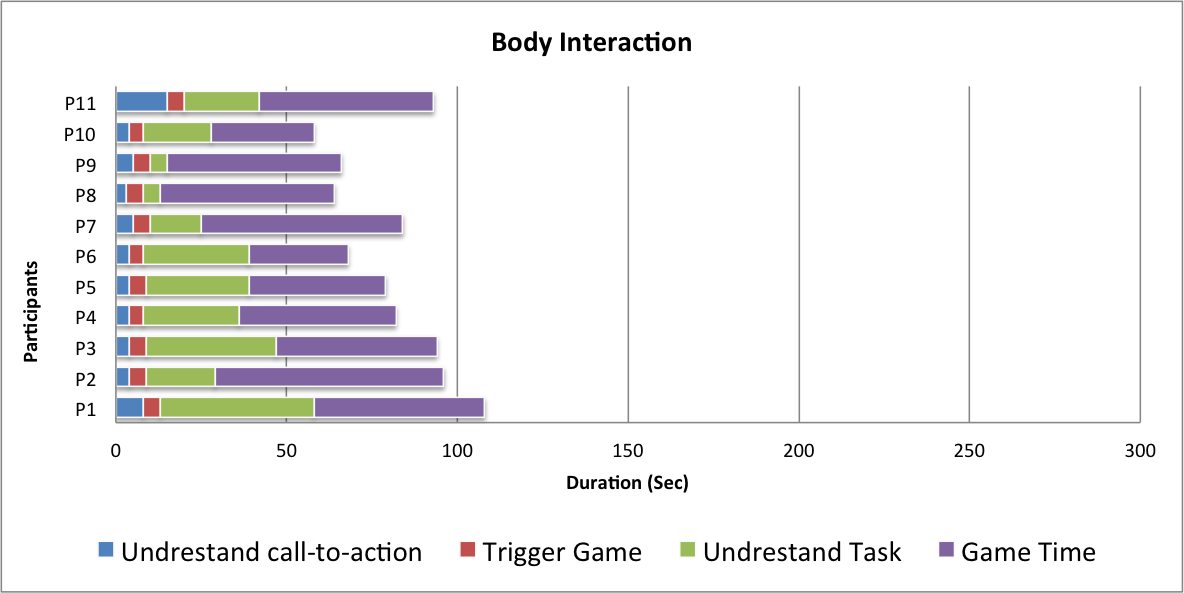
\includegraphics[width=\textwidth,height=0.35\textheight]{Appendices/6/body_performance}%
    \caption{Pariticipant's body performance}%
    \label{app:body_performance}%
\end{figure}


\subsection{Mobile}
\begin{figure}[H]
    \centering
    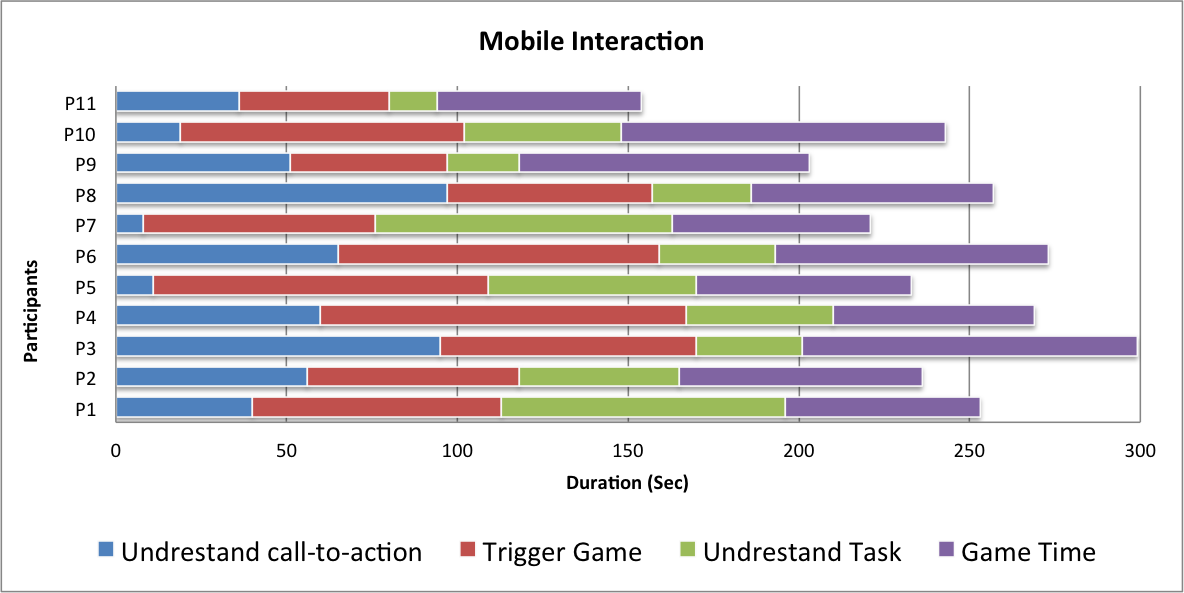
\includegraphics[width=\textwidth,height=0.35\textheight]{Appendices/6/mobile_performance}%
    \caption{Pariticipant's mobile performance}%
    \label{app:mobile_performance}%
\end{figure}

\newpage
\chapter{Field Study}

\setcounter{figure}{0}
\setcounter{table}{0}

\section{Interview Questionnaire}


\begin{figure}[H]
 \centering 
    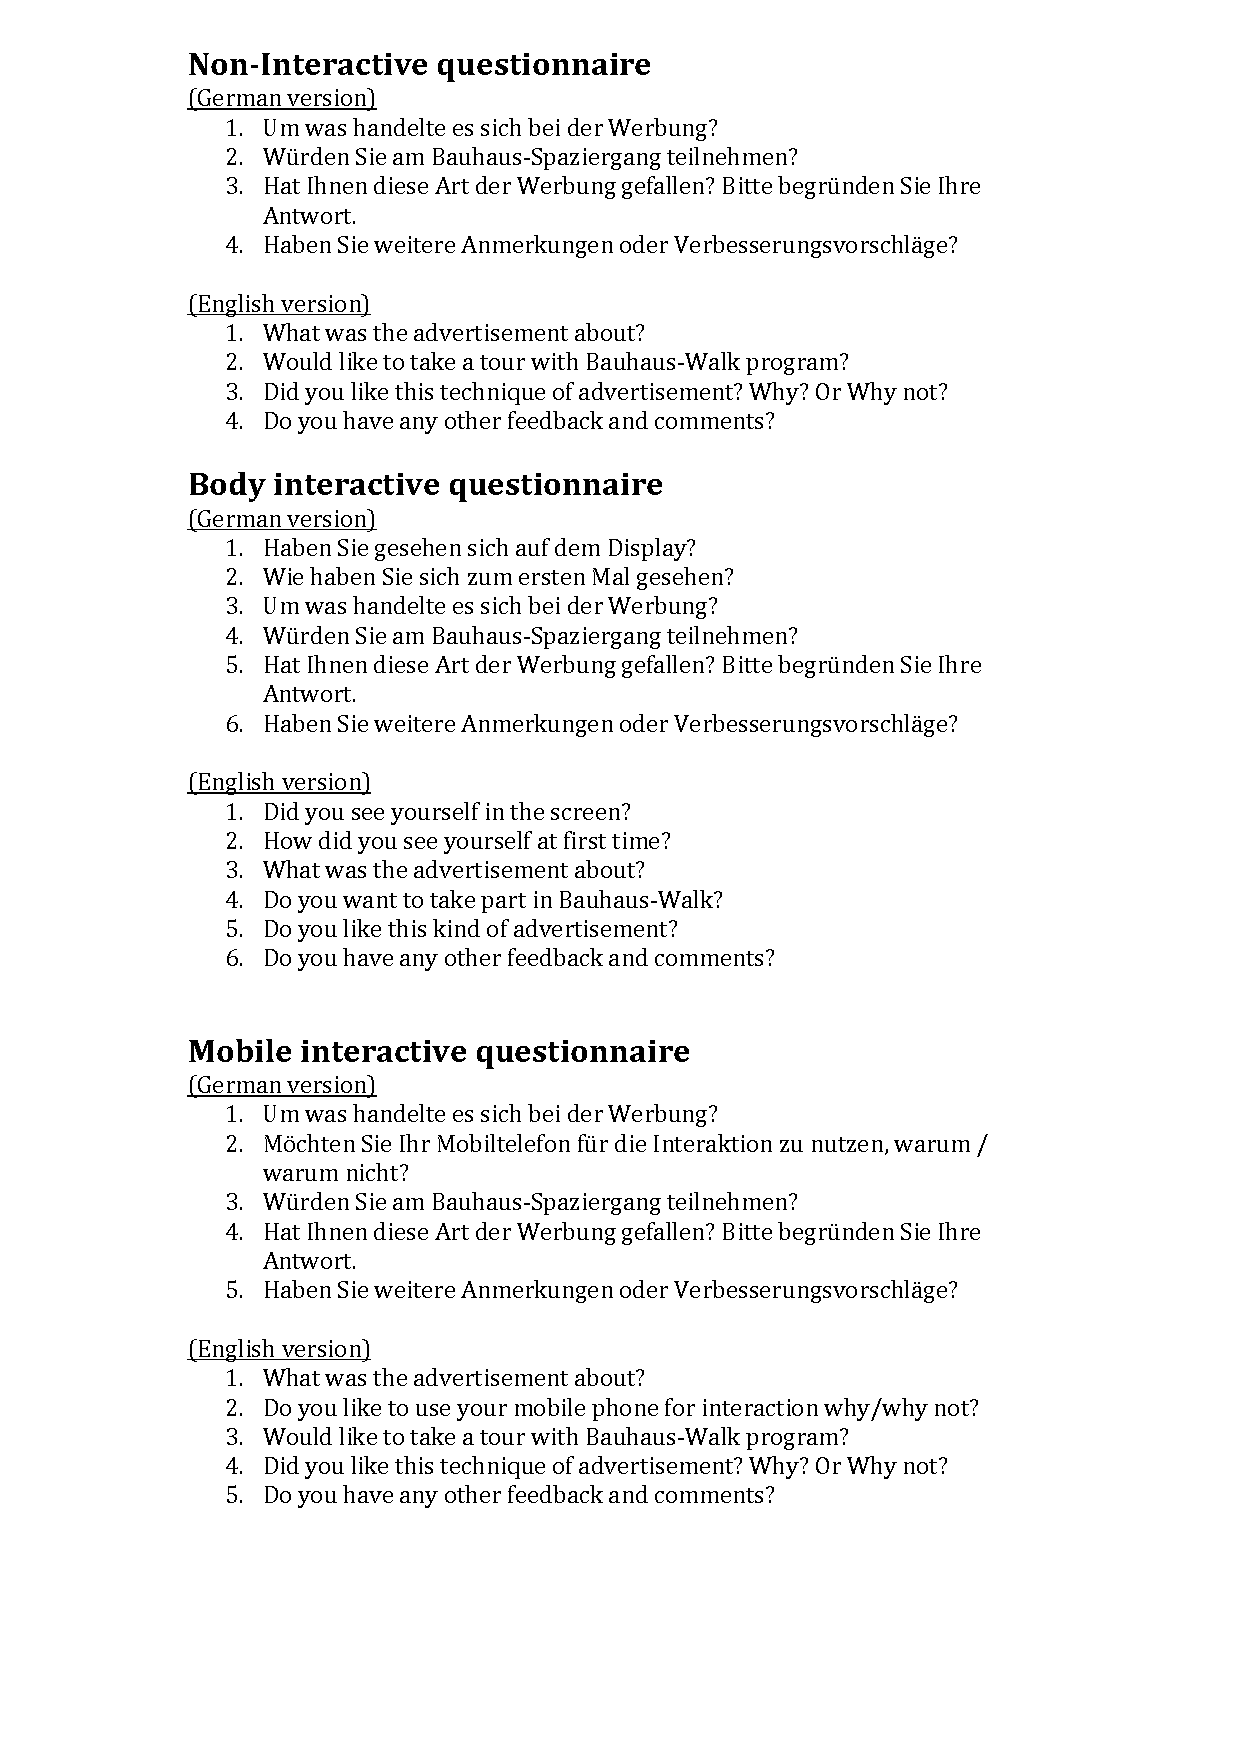
\includegraphics[width=\textwidth,height=0.8\textheight]{Appendices/8/whole_week_interivew.pdf}
    \caption{Interview questions for all conditions.}
     \label{app:whole_interview}%
\end{figure}


\section{Non-Interactive glance count}

\begin{figure}[H]
 \centering 
    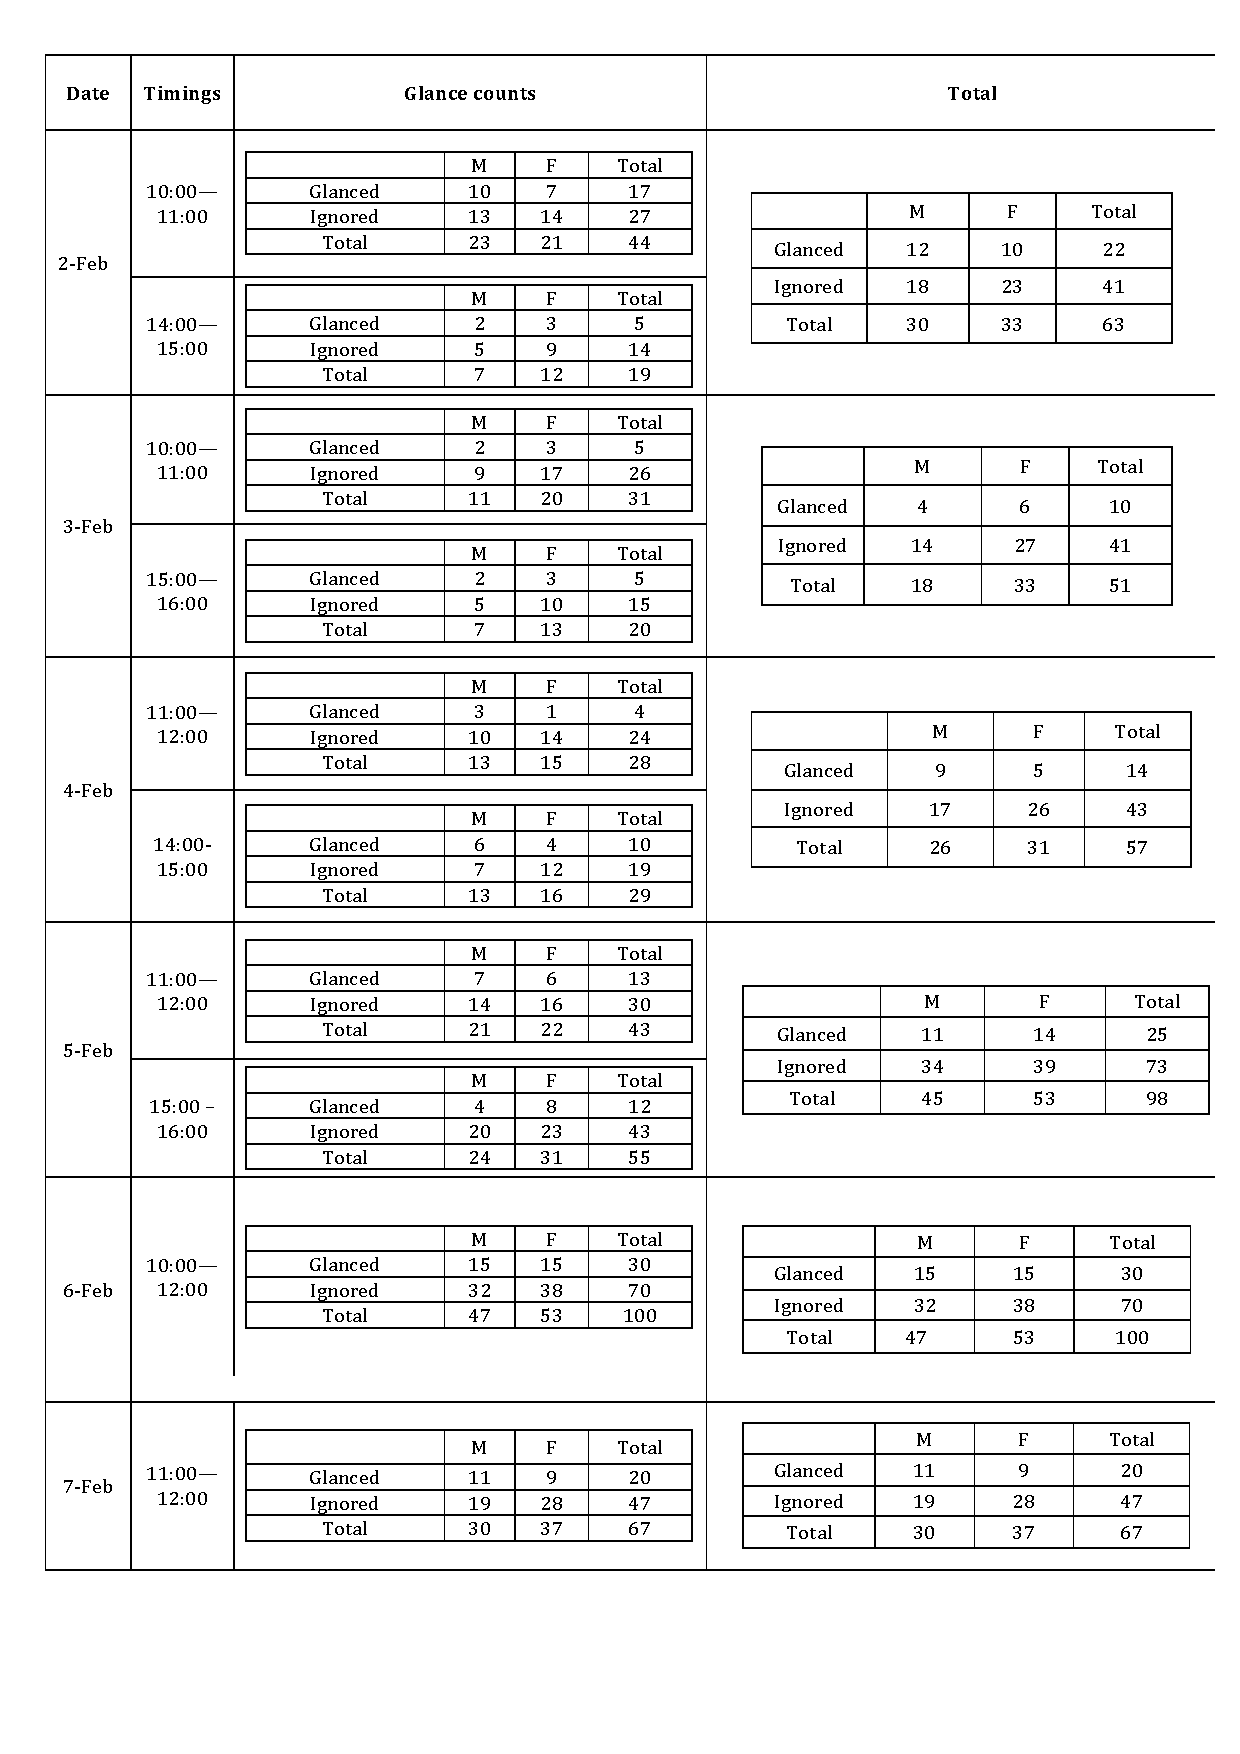
\includegraphics[width=\textwidth,height=0.8\textheight]{Appendices/8/non-interactive/non-interactive_glances.pdf}
    \caption{Non-interactive glance counts}
     \label{app:non-interactive-glancecount}%
\end{figure}


\section{Body Interactive glance count}

\begin{figure}[H]
 \centering 
    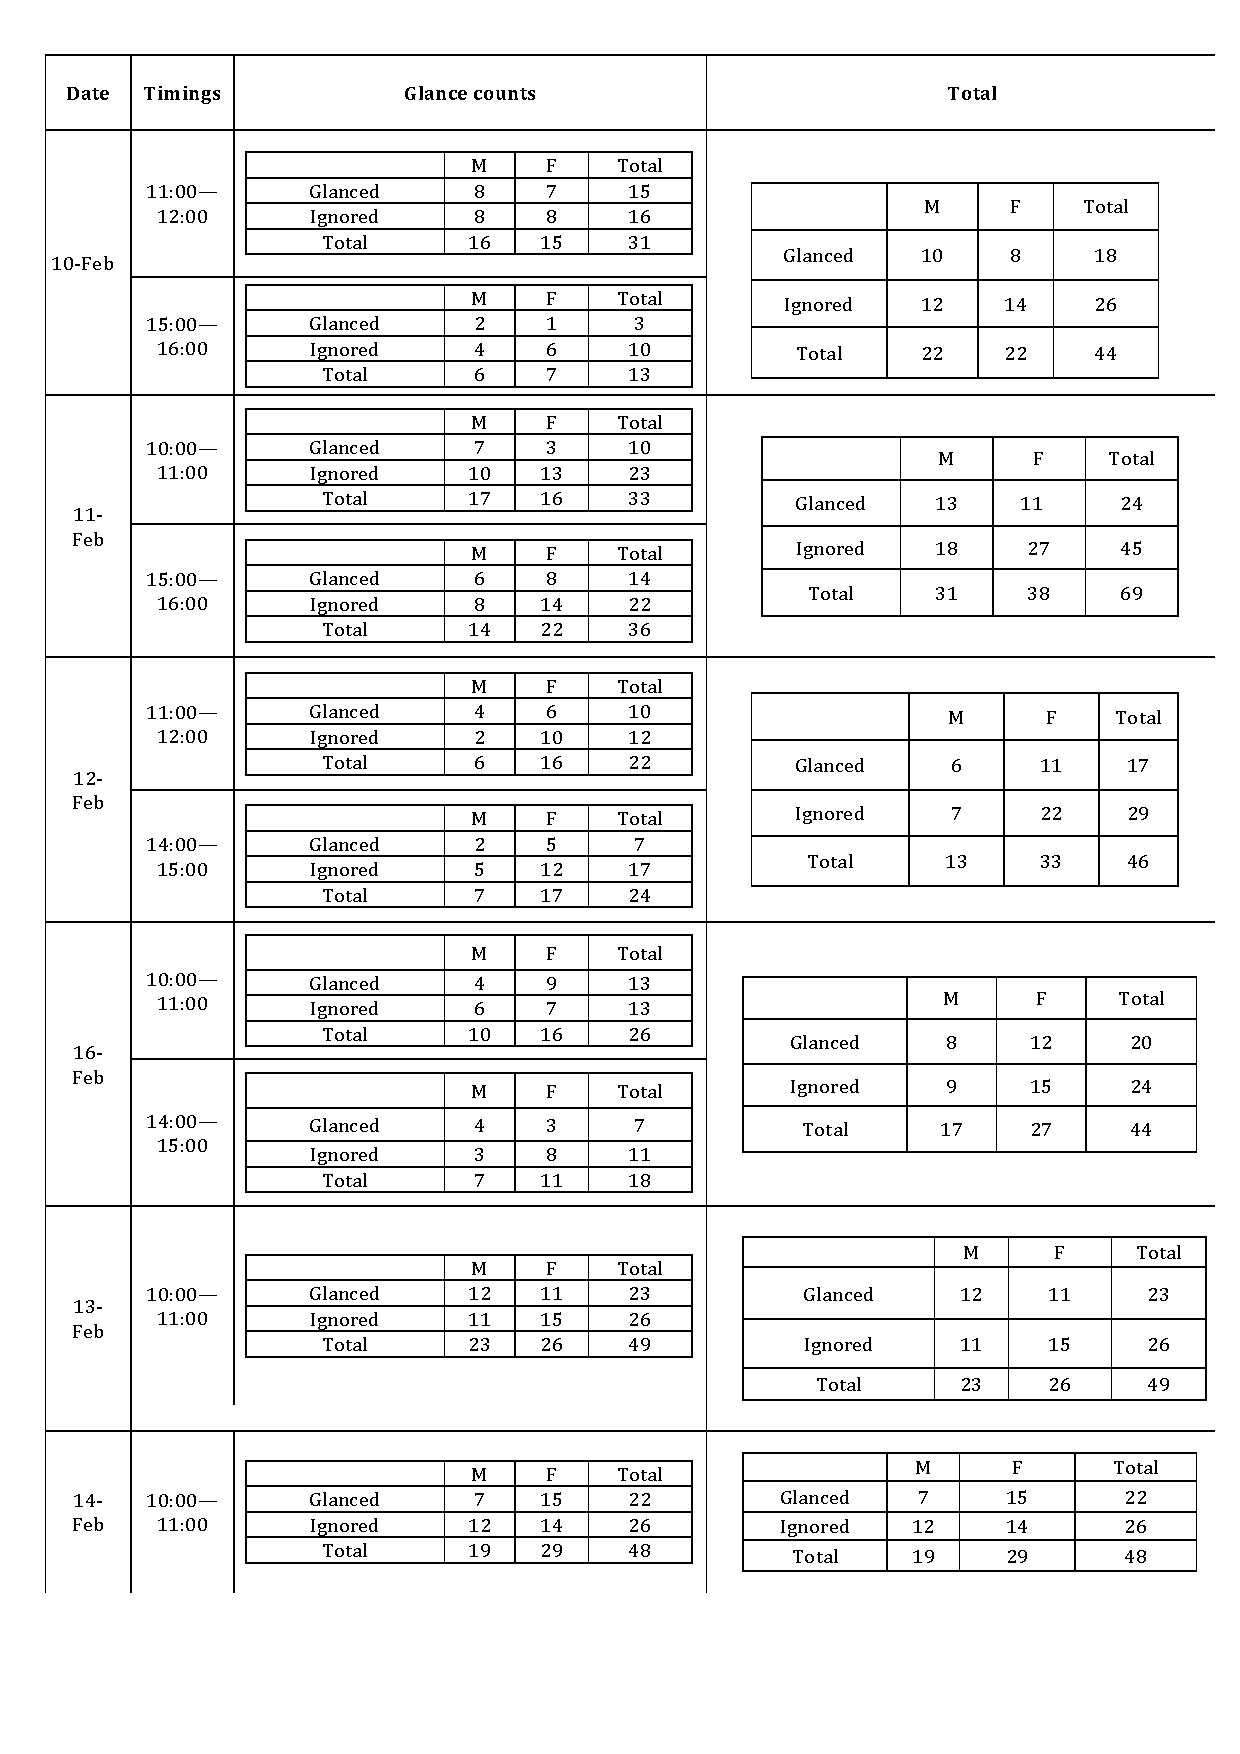
\includegraphics[width=\textwidth,height=0.8\textheight]{Appendices/8/body-interactive/body-interactive_glances.pdf}
    \caption{Body interactive glance counts}
     \label{app:body-interactive-glancecount}%
\end{figure}



\section{Body Interactive glance count}

\begin{figure}[H]
 \centering 
    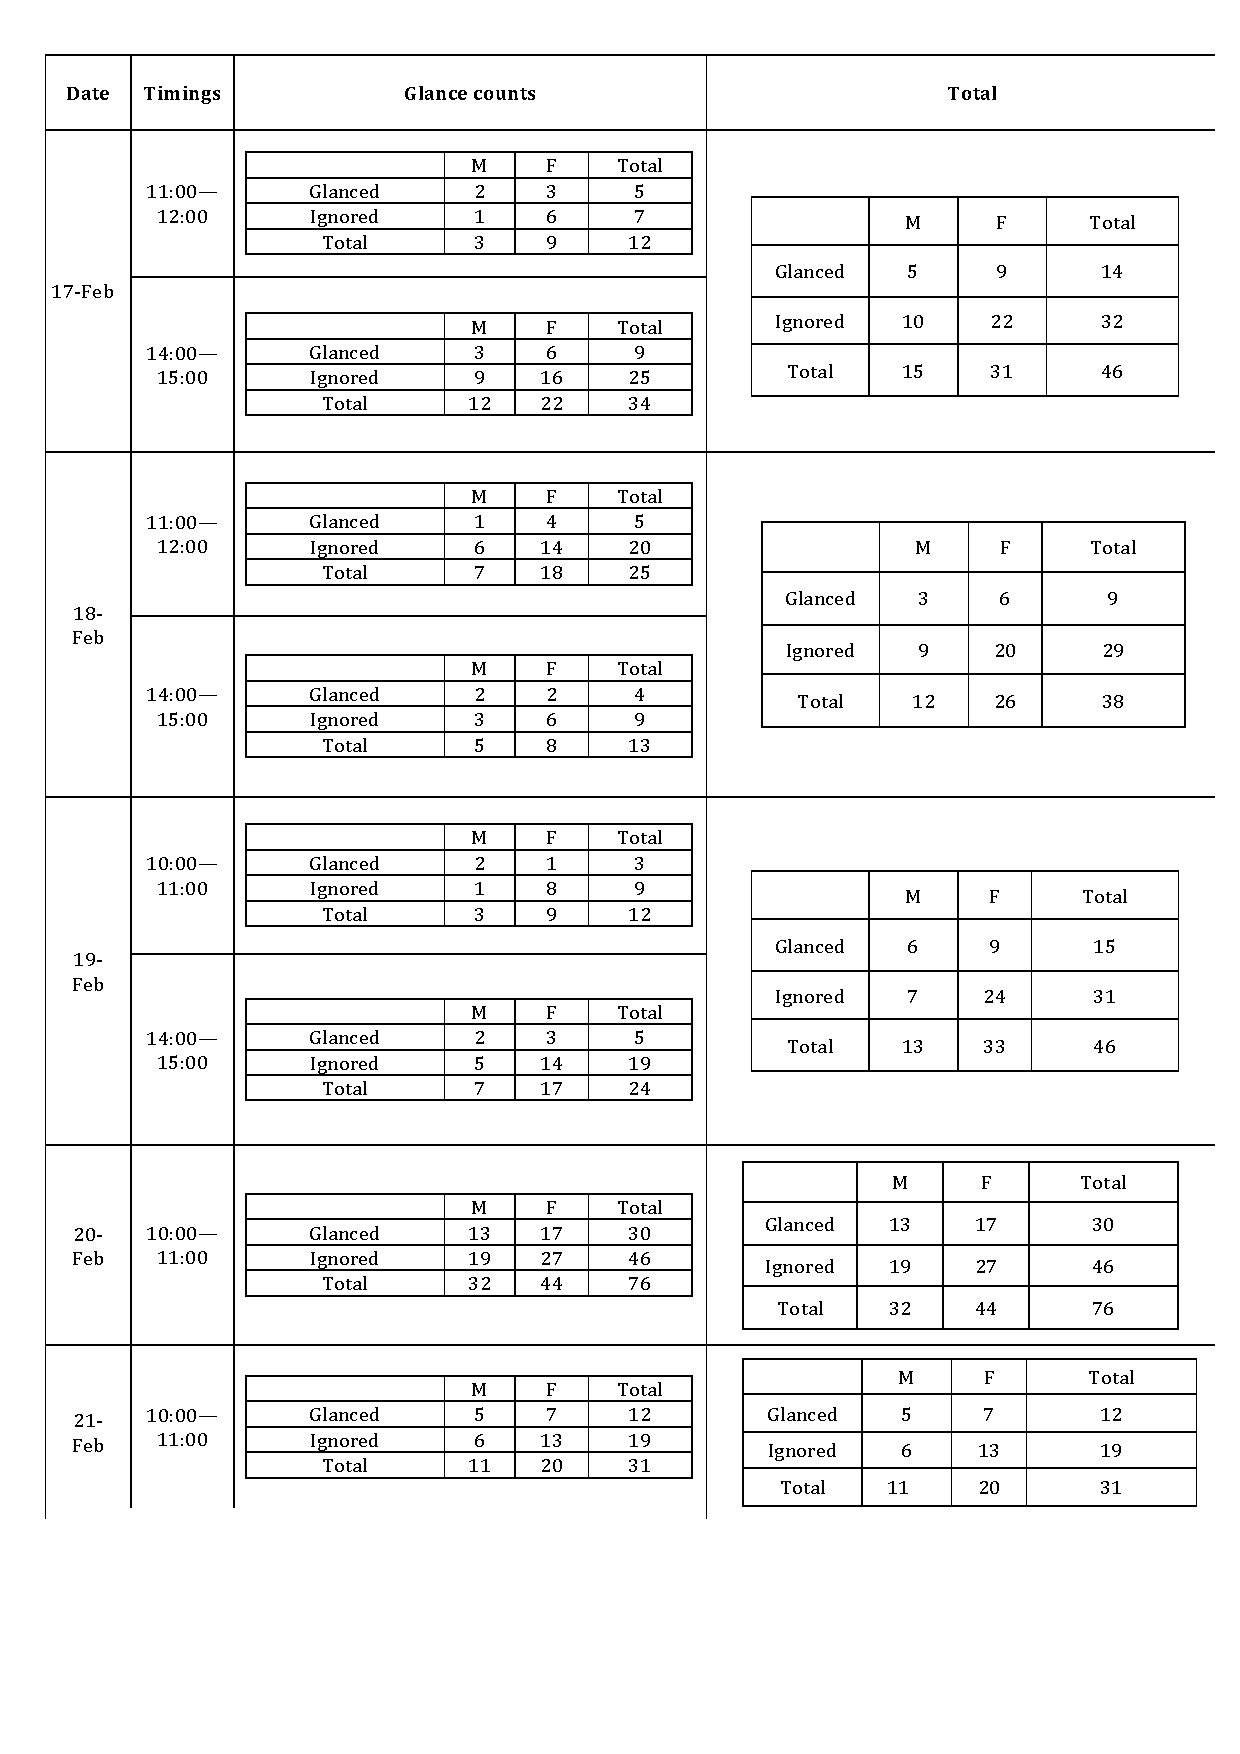
\includegraphics[width=\textwidth,height=0.8\textheight]{Appendices/8/mobile-interactive/mobile-interactive_glances.pdf}
   \caption{Mobile interactive glance counts}
     \label{app:mobile-interactive-glancecount}%
\end{figure}



\section{Non-Interactive interview code}
\begin{minipage}{1.14\textwidth}
\begin{flushleft} 
\begin{figure}[H]
 \centering 
    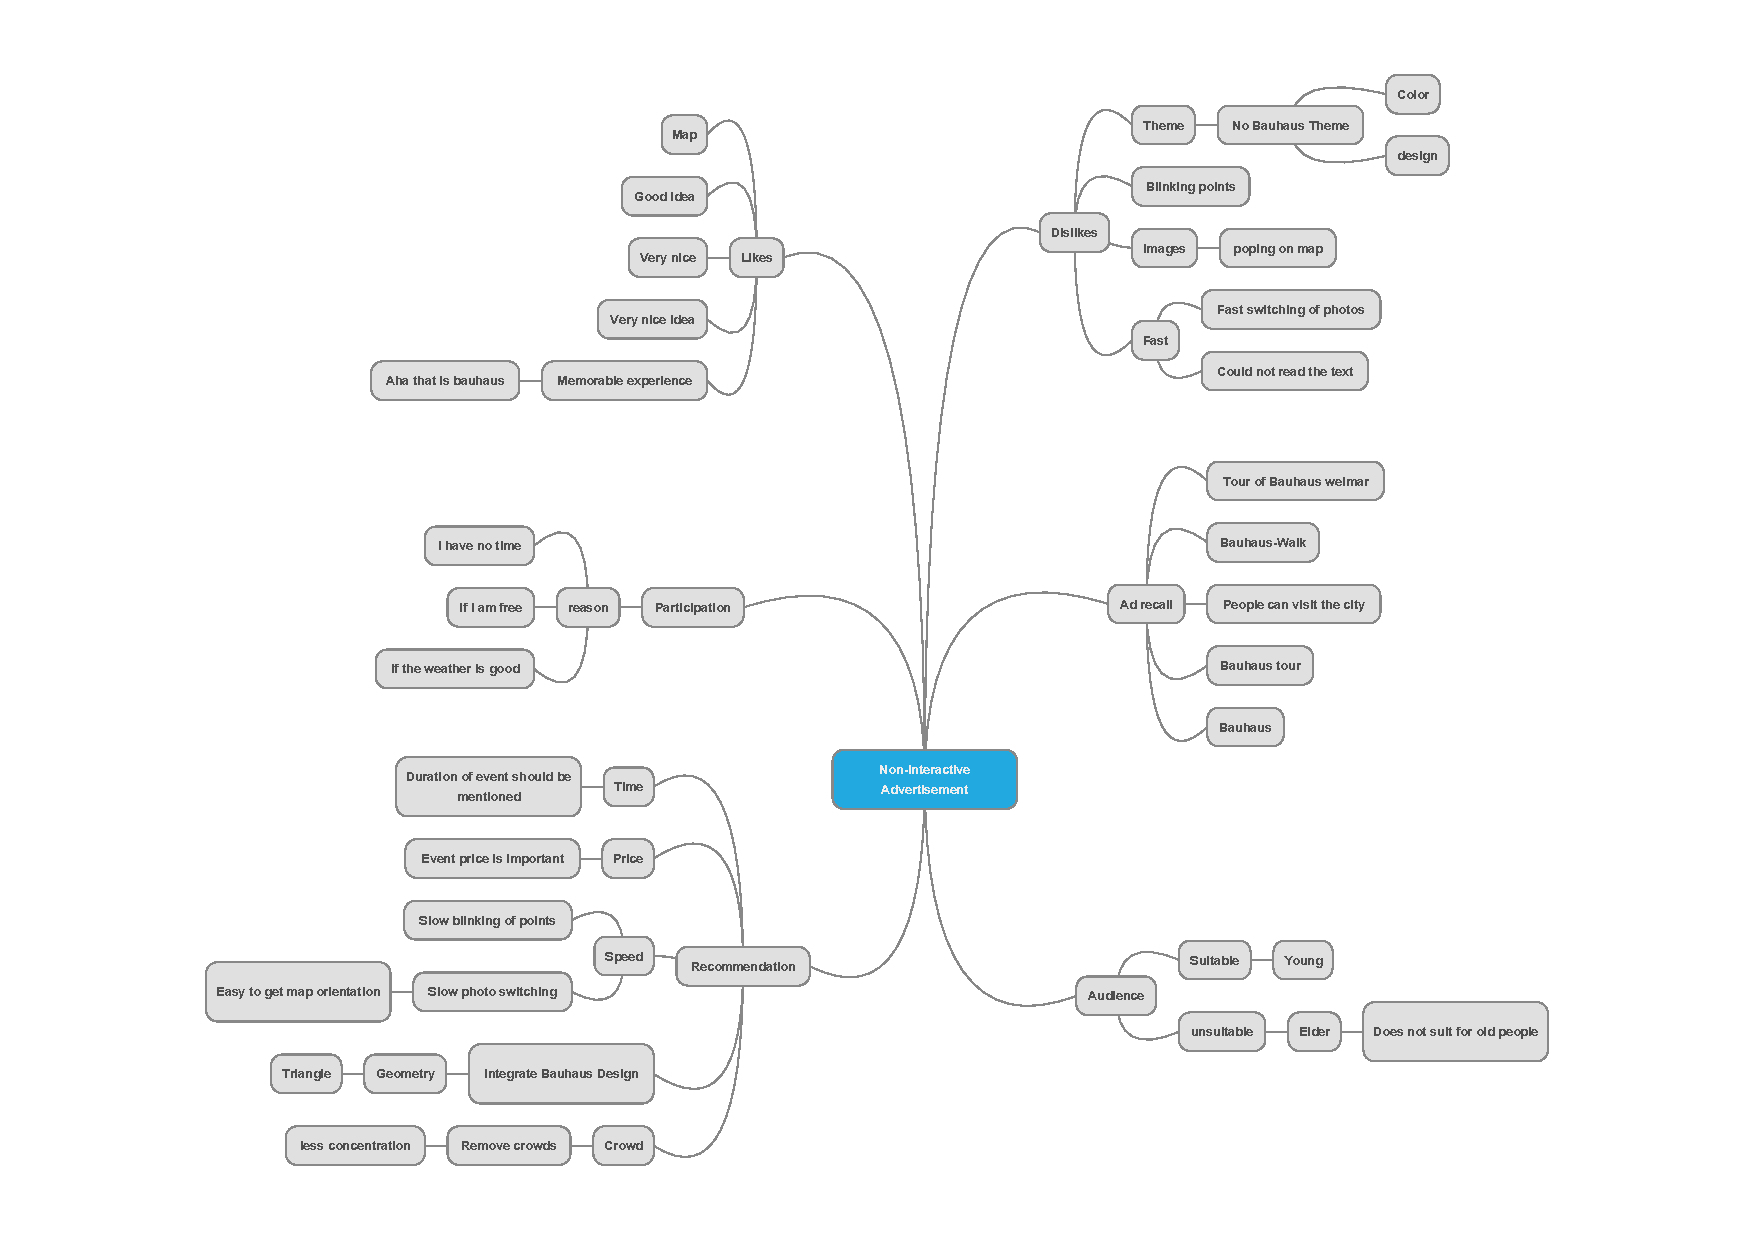
\includegraphics[width = \textwidth, height=0.8\textheight]{Appendices/8/non-interactive/non-interactive_code.pdf}
    \caption{Non-Interactive interview code}
     \label{app:non-interactiveinterviewcode_}%
\end{figure}
\end{flushleft} 
\end{minipage}


\section{Body Interactive interview code}
\begin{minipage}{1.14\textwidth}
\begin{flushleft} 
\begin{figure}[H]
 \centering 
    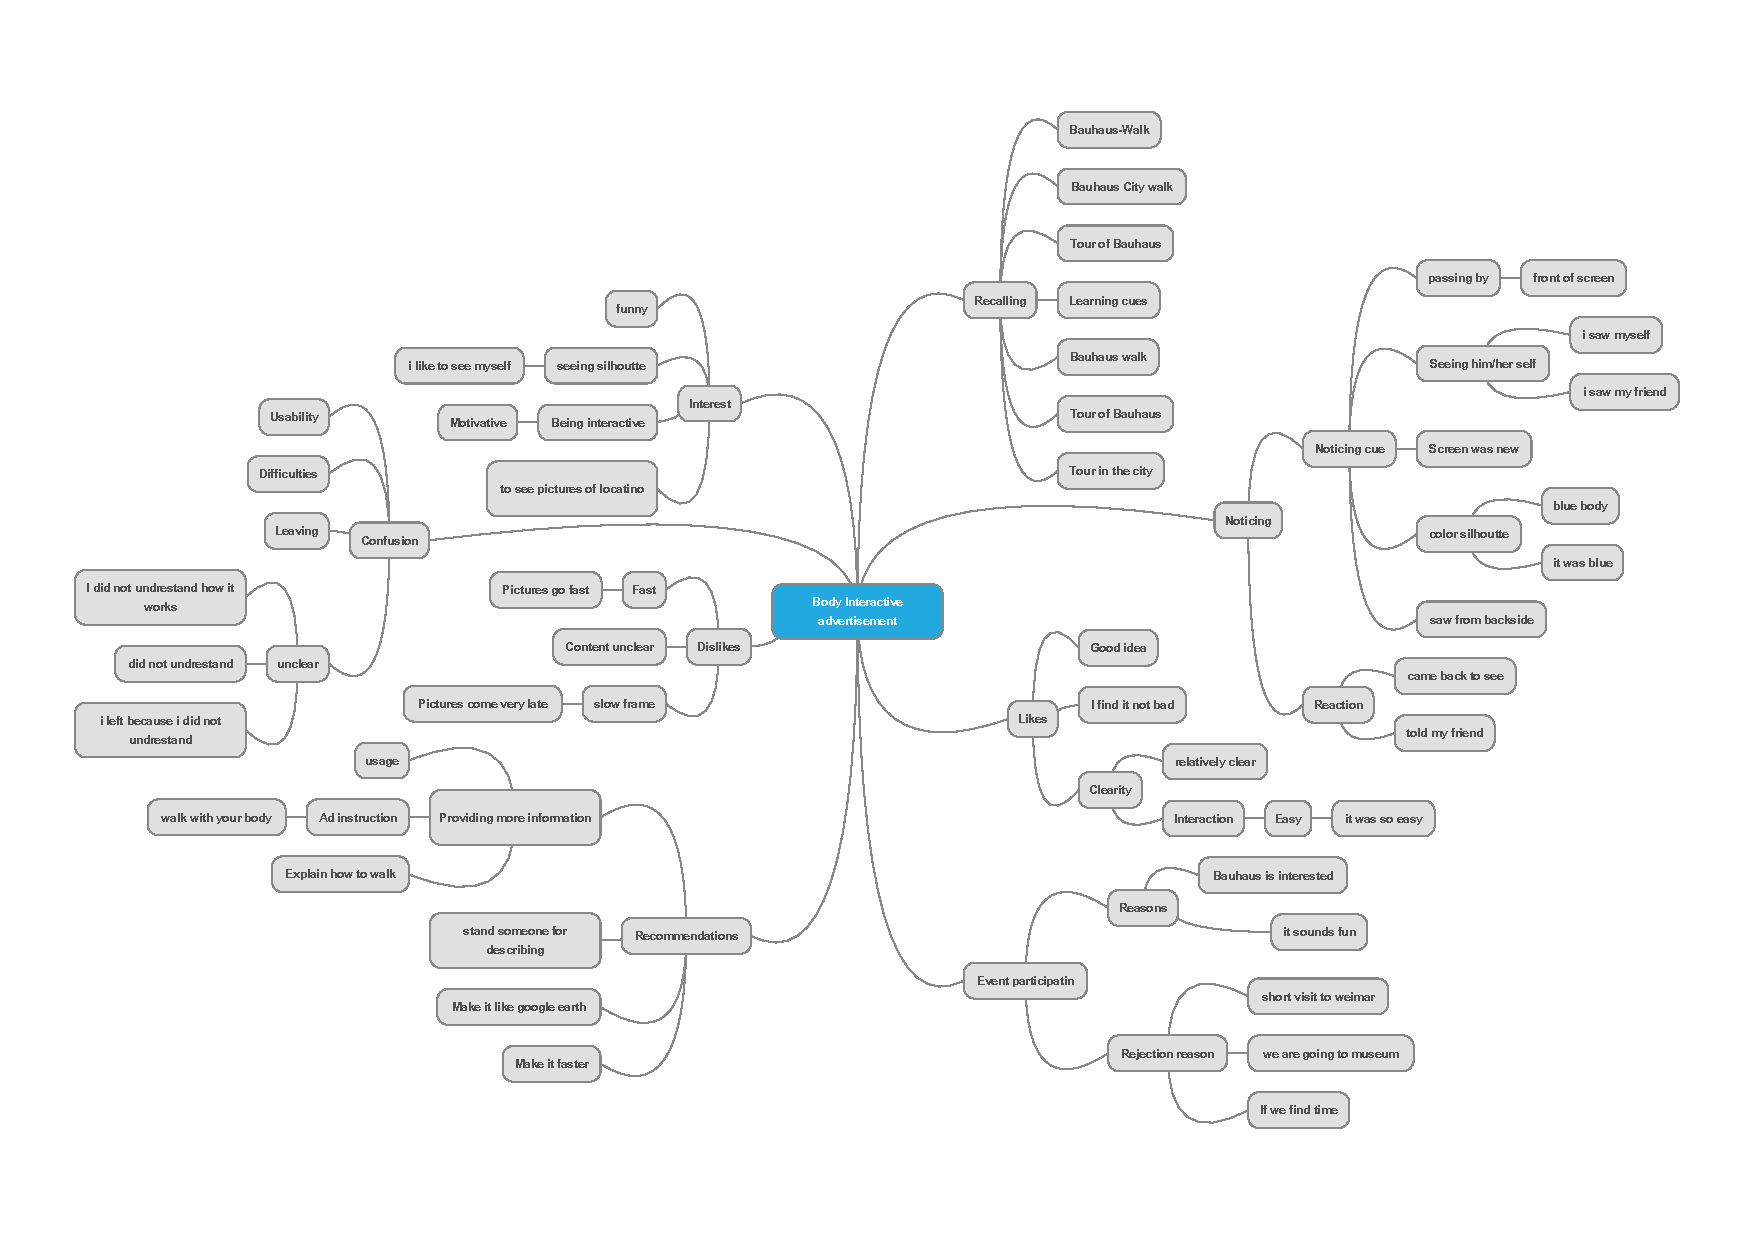
\includegraphics[width = \textwidth, height=0.8\textheight]{Appendices/8/body-interactive/body-Interactive_code.pdf}
    \caption{Body Interactive interview code}
     \label{app:body-interactiveinterviewcode_}%
\end{figure}
\end{flushleft} 
\end{minipage}



\section{Mobile Interactive interview code}
\begin{minipage}{1.14\textwidth}
\begin{flushleft} 
\begin{figure}[H]
 \centering 
    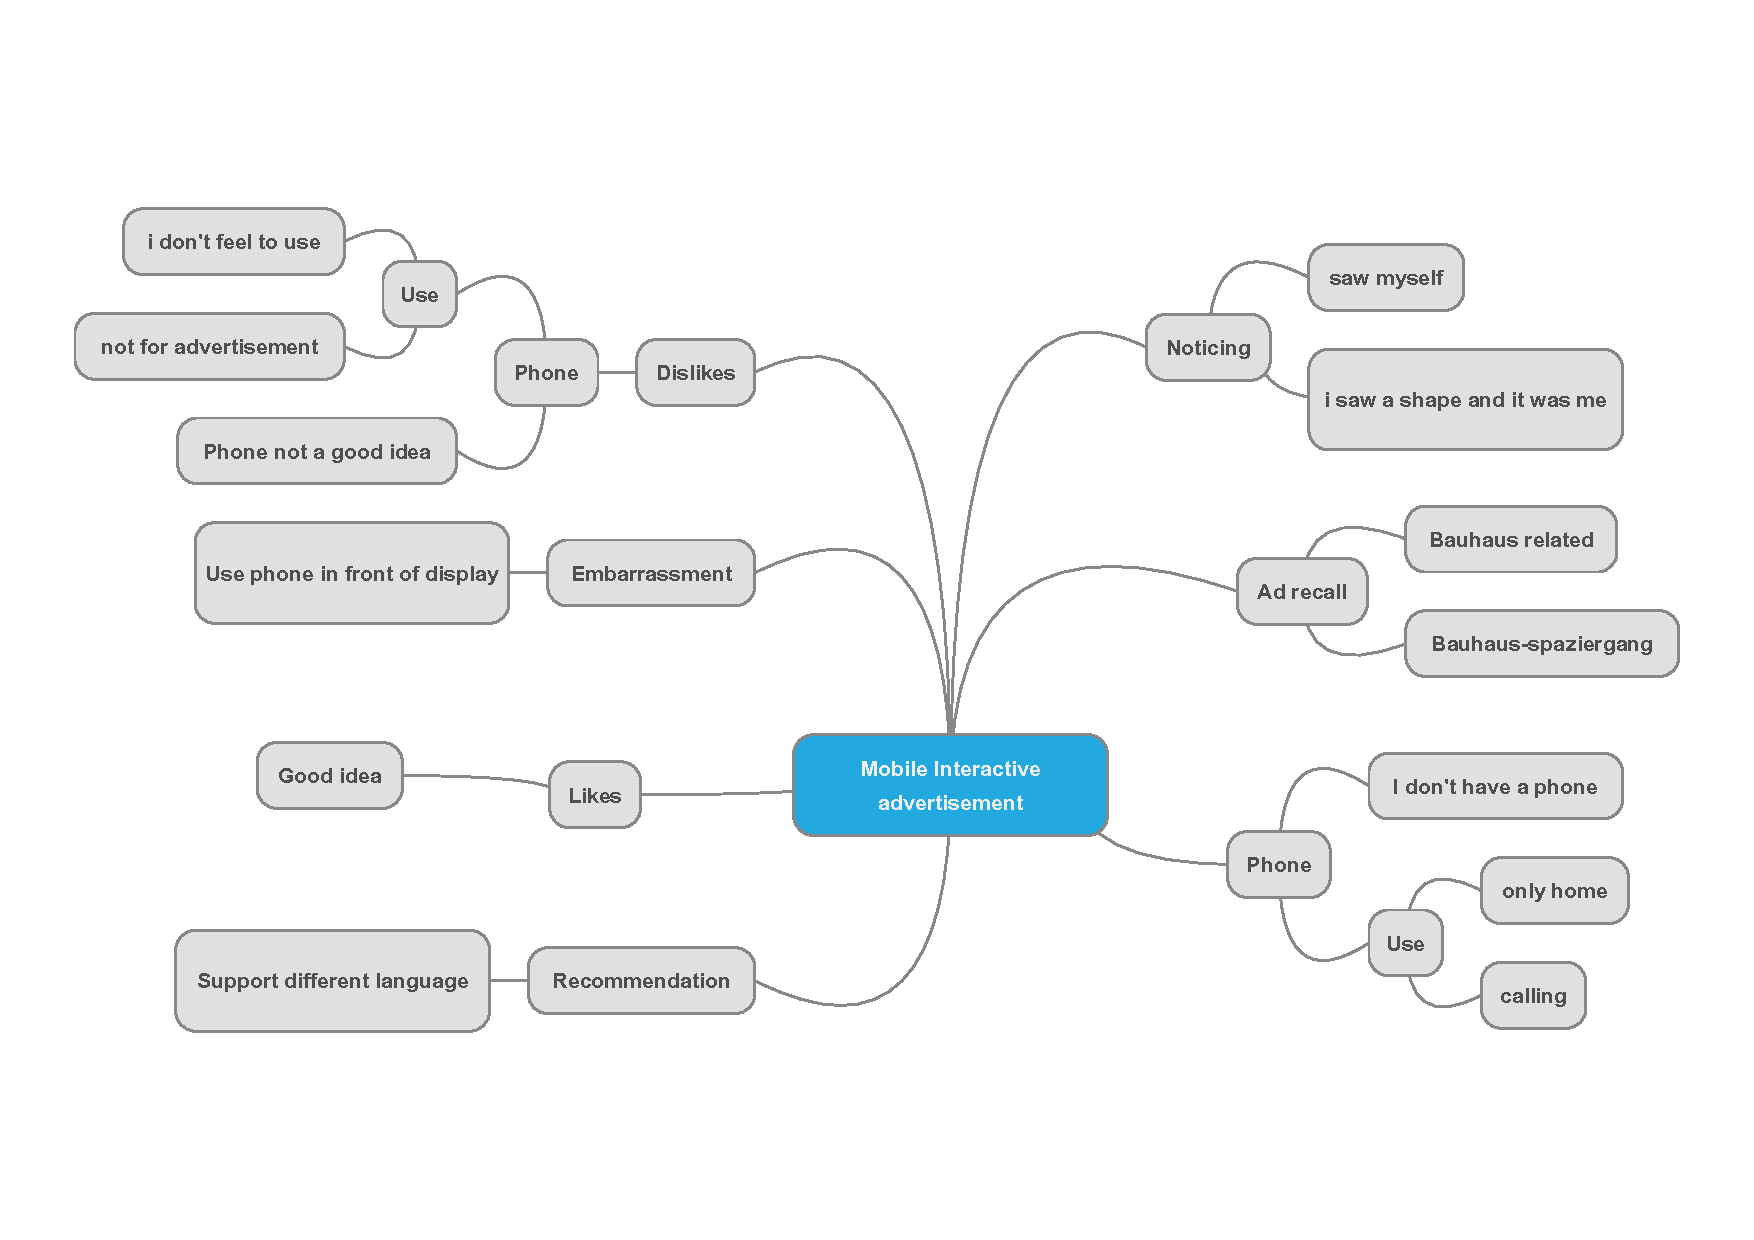
\includegraphics[width = \textwidth, height=0.8\textheight]{Appendices/8/mobile-interactive/mobile-Interactive_code.pdf}
    \caption{Mobile Interactive interview code}
     \label{app:mobile-interactiveinterviewcode_}%
\end{figure}
\end{flushleft} 
\end{minipage}

% Observation notes
\section{Non-Interactive observation notes}
\begin{figure}[H]
 \centering 
    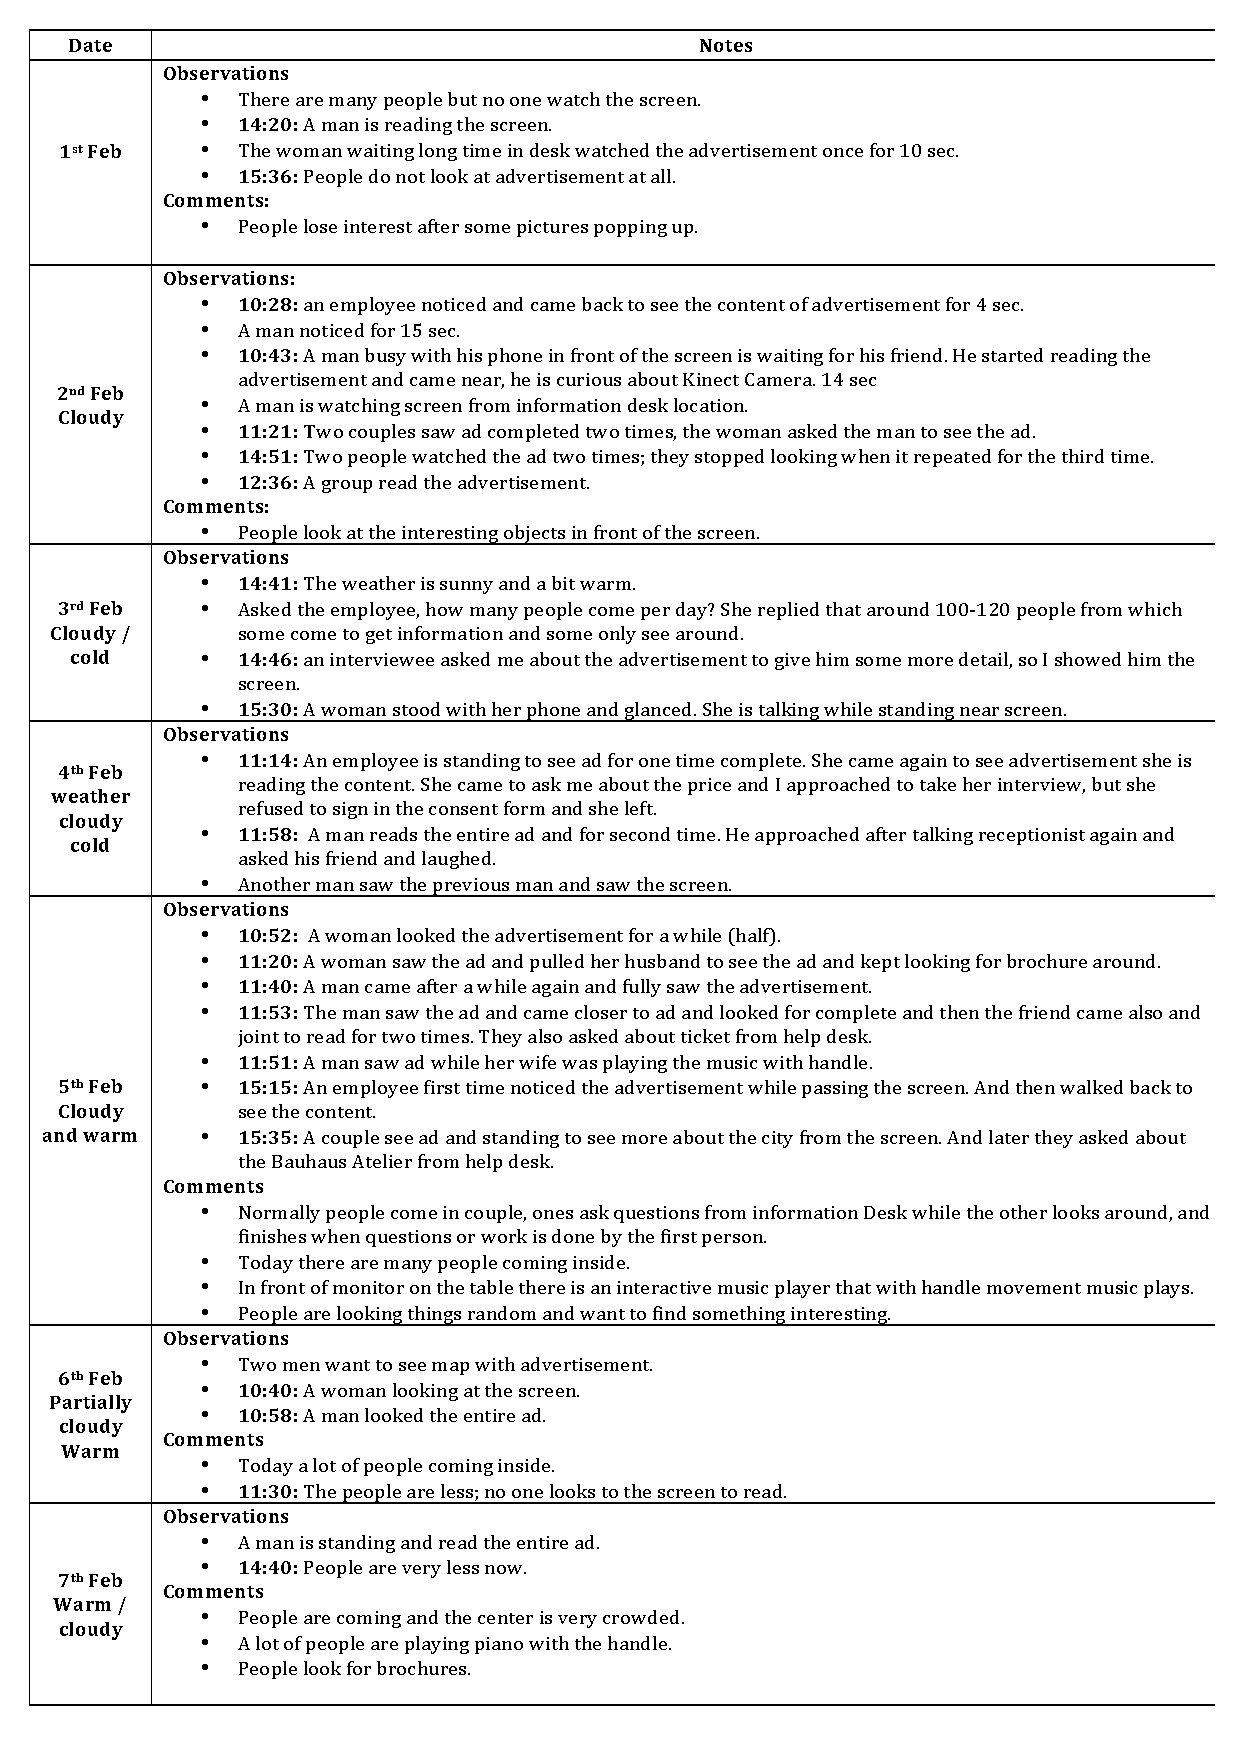
\includegraphics[width=\textwidth,height=0.8\textheight]{Appendices/8/non-interactive/Observation_notes.pdf}
    \caption{Non-Interactive observation notes}
     \label{app:Non-Interactiveobservation-notes}%
\end{figure}


\section{Body Interactive observation notes}
\begin{figure}[H]
 \centering 
    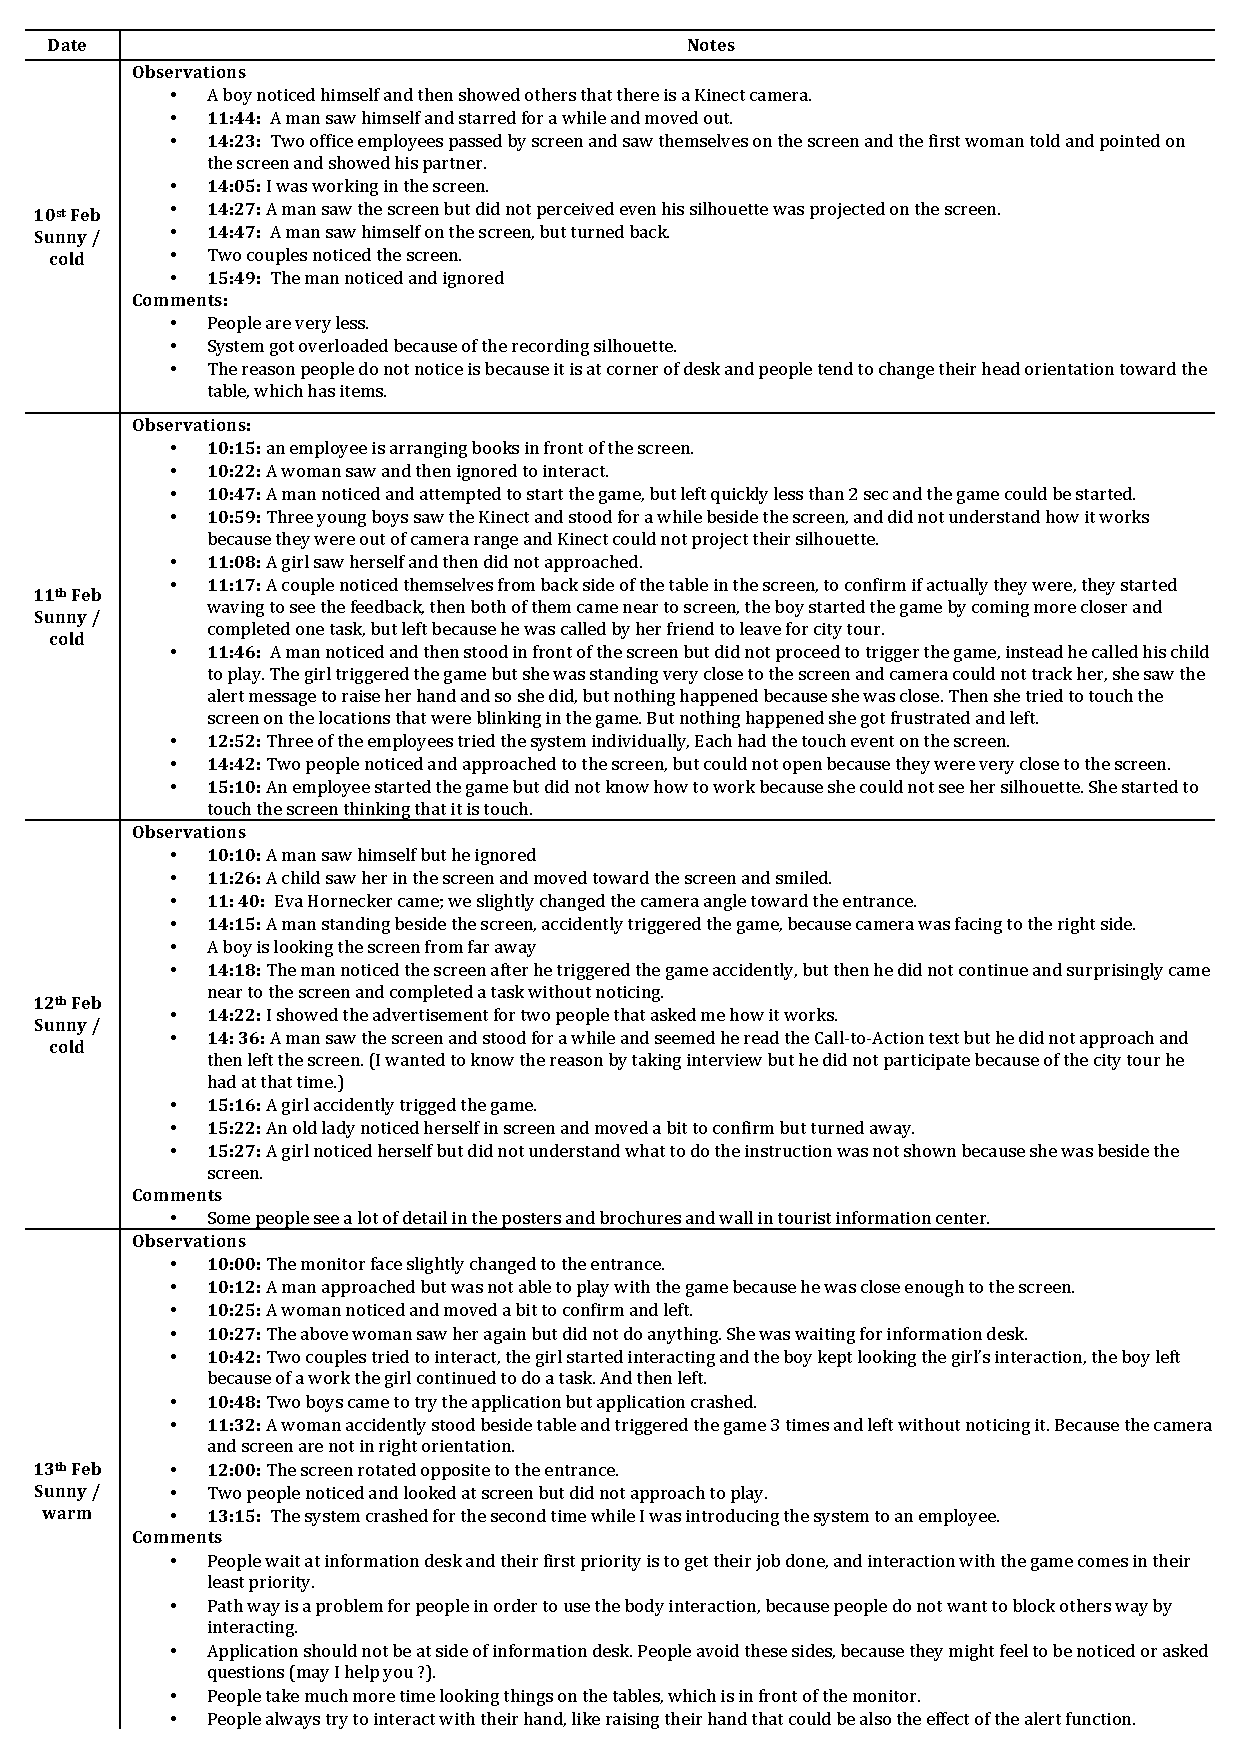
\includegraphics[width=\textwidth,height=0.8\textheight]{Appendices/8/body-interactive/Note_1.pdf}
    \caption{Body Interactive observation notes (1)}
     \label{app:body-Interactiveobservation-notes1}%
\end{figure}


\begin{figure}[H]
 \centering 
    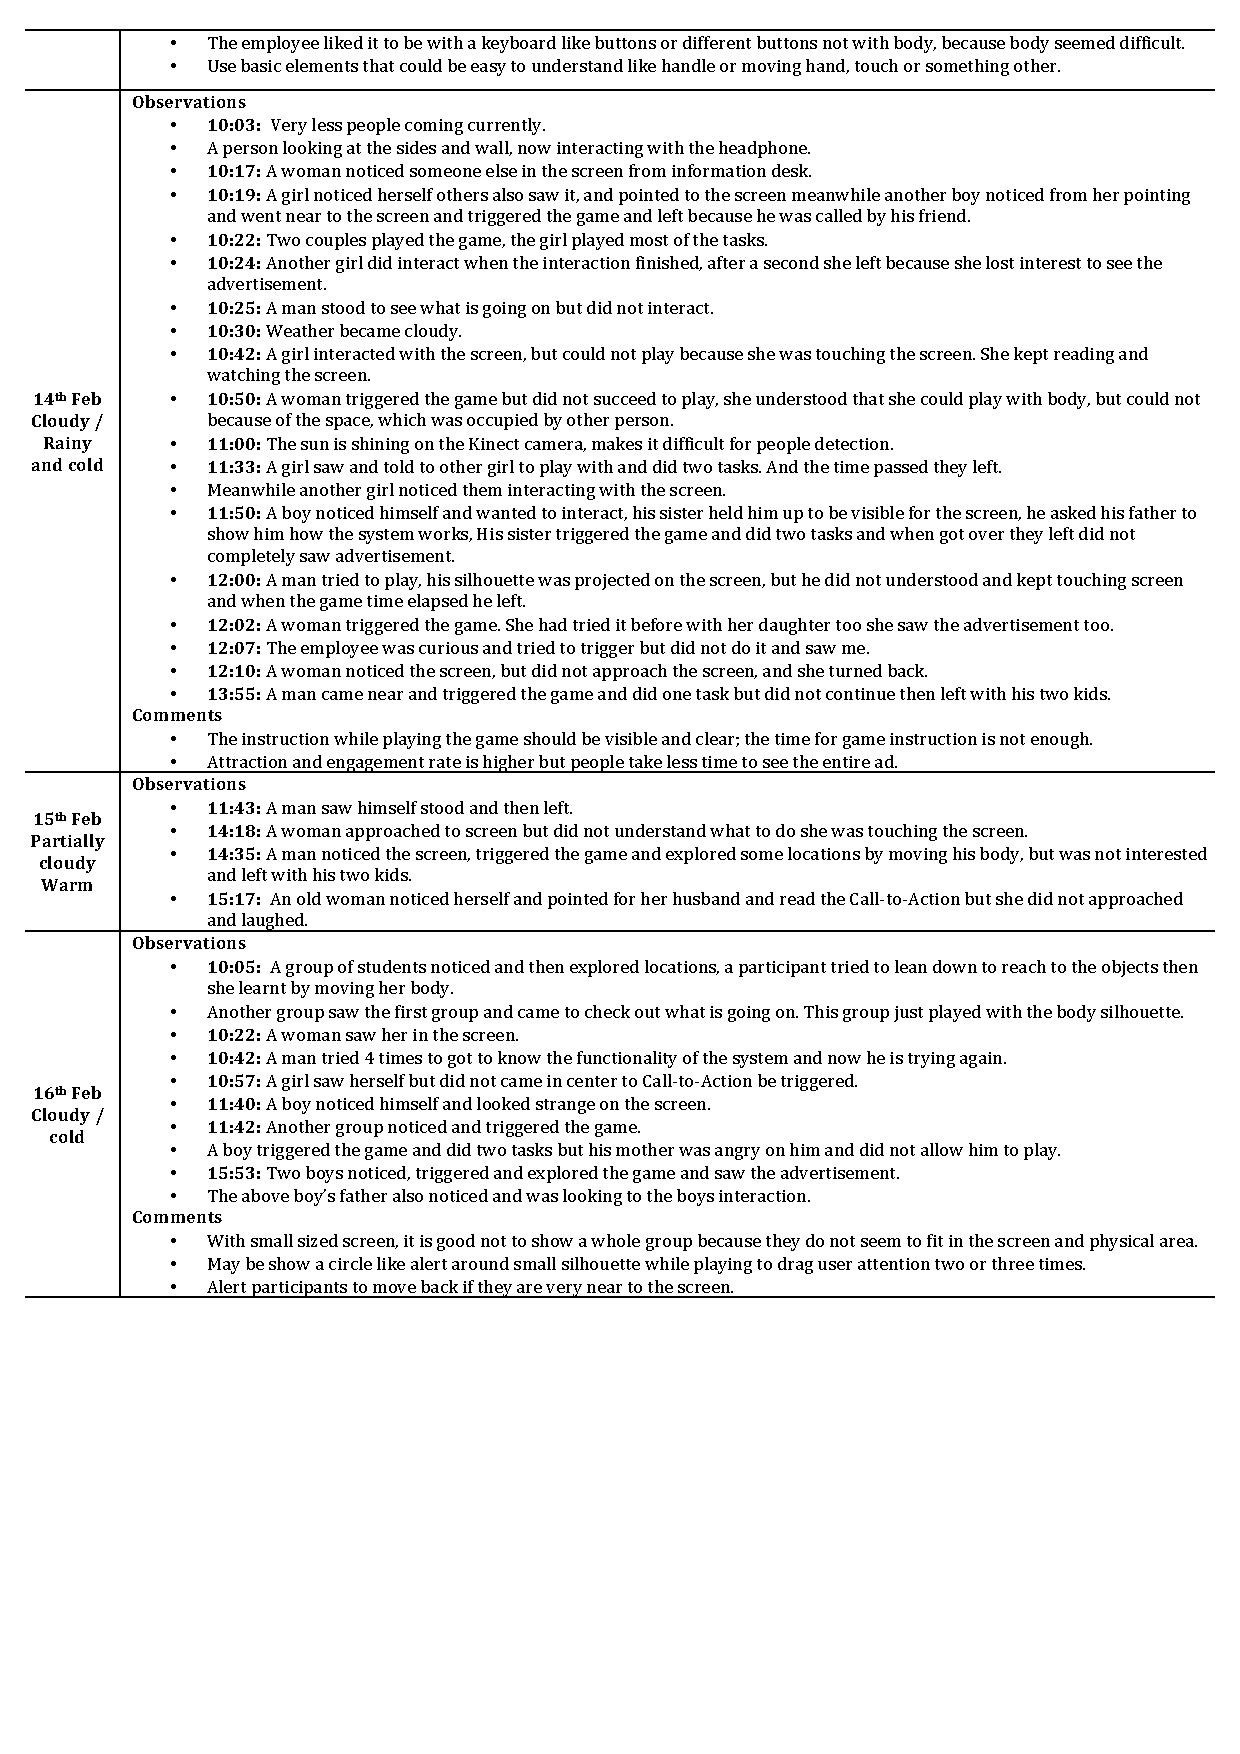
\includegraphics[width=\textwidth,height=0.8\textheight]{Appendices/8/body-interactive/Note_2.pdf}
    \caption{Body Interactive observation notes (2)}
     \label{app:body-Interactiveobservation-notes2}%
\end{figure}


\section{Mobile Interactive observation notes}
\begin{figure}[H]
 \centering 
    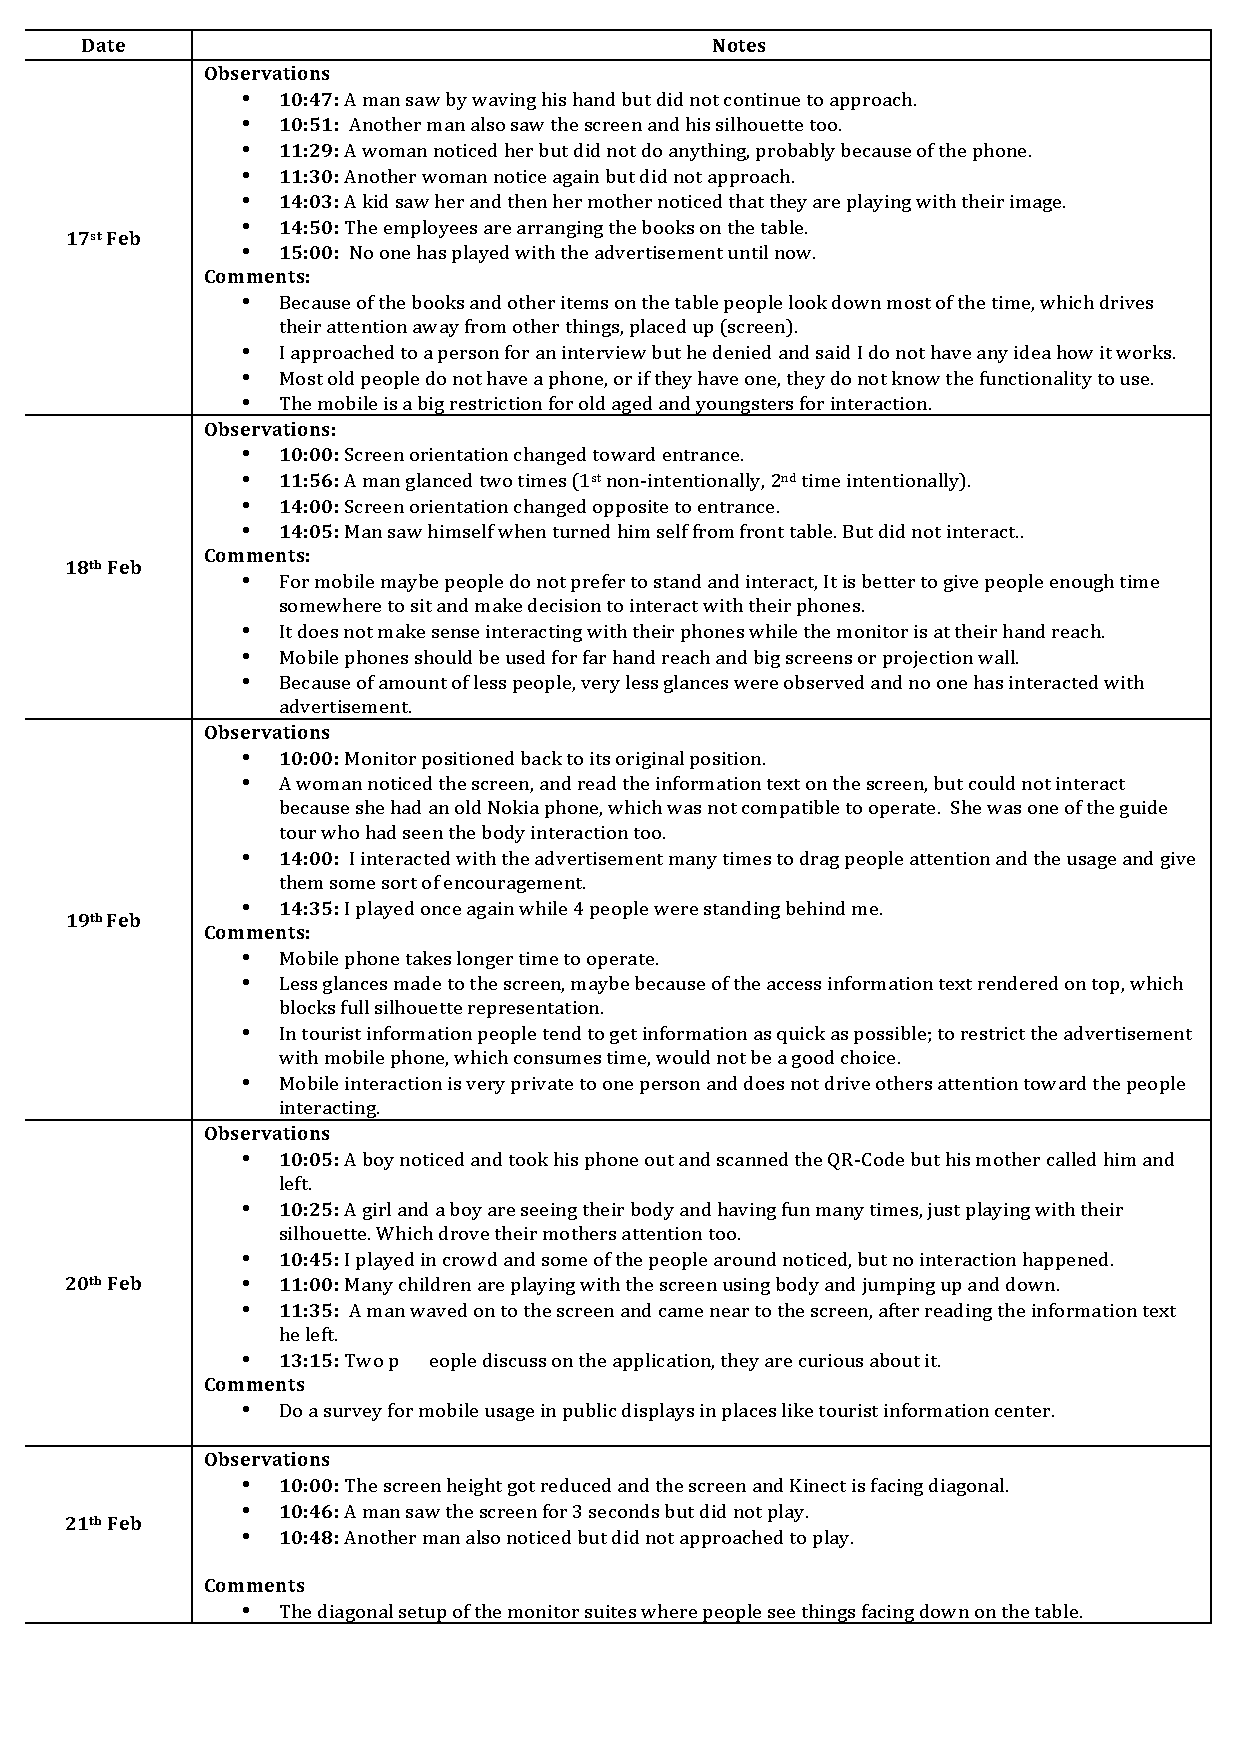
\includegraphics[width=\textwidth,height=0.8\textheight]{Appendices/8/mobile-interactive/notetaking.pdf}
    \caption{Mobile Interactive observation notes}
     \label{app:MobileInteractiveobservation-notes}%
\end{figure}



\chapter{Enhanced body interactive Field Study}
\setcounter{figure}{0}
\setcounter{table}{0}
    
\section{Enhanced Interactive advertisement Glance count}

\begin{figure}[H]
 \centering 
    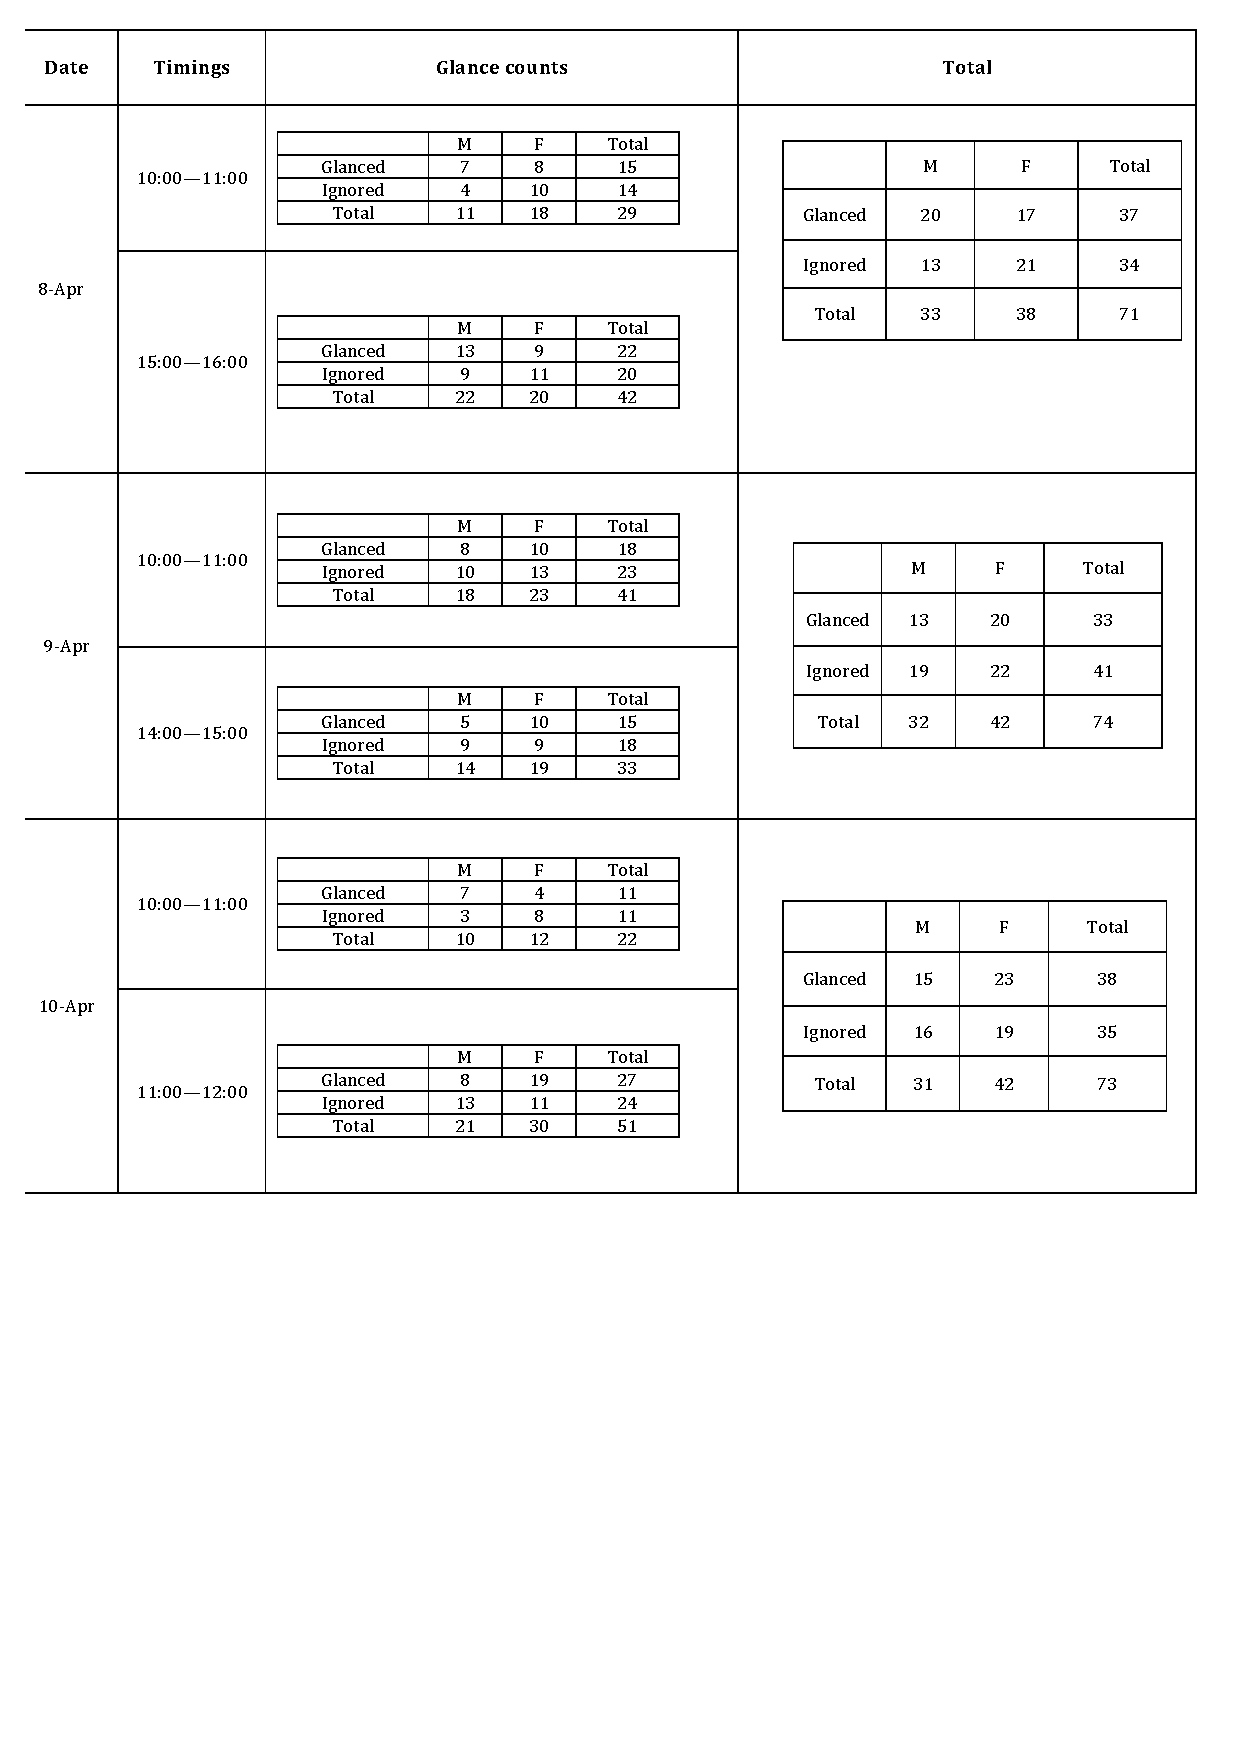
\includegraphics[width=\textwidth,height=0.5\textheight]{Appendices/9/new_body_glance.pdf}
    \caption{Enhanced Interactive advertisement Glance count}
     \label{app:EnhancedInteractiveadvertisementGlance}%
\end{figure}


\section{Enhanced Interactive observation notes}

\begin{figure}[H]
 \centering 
    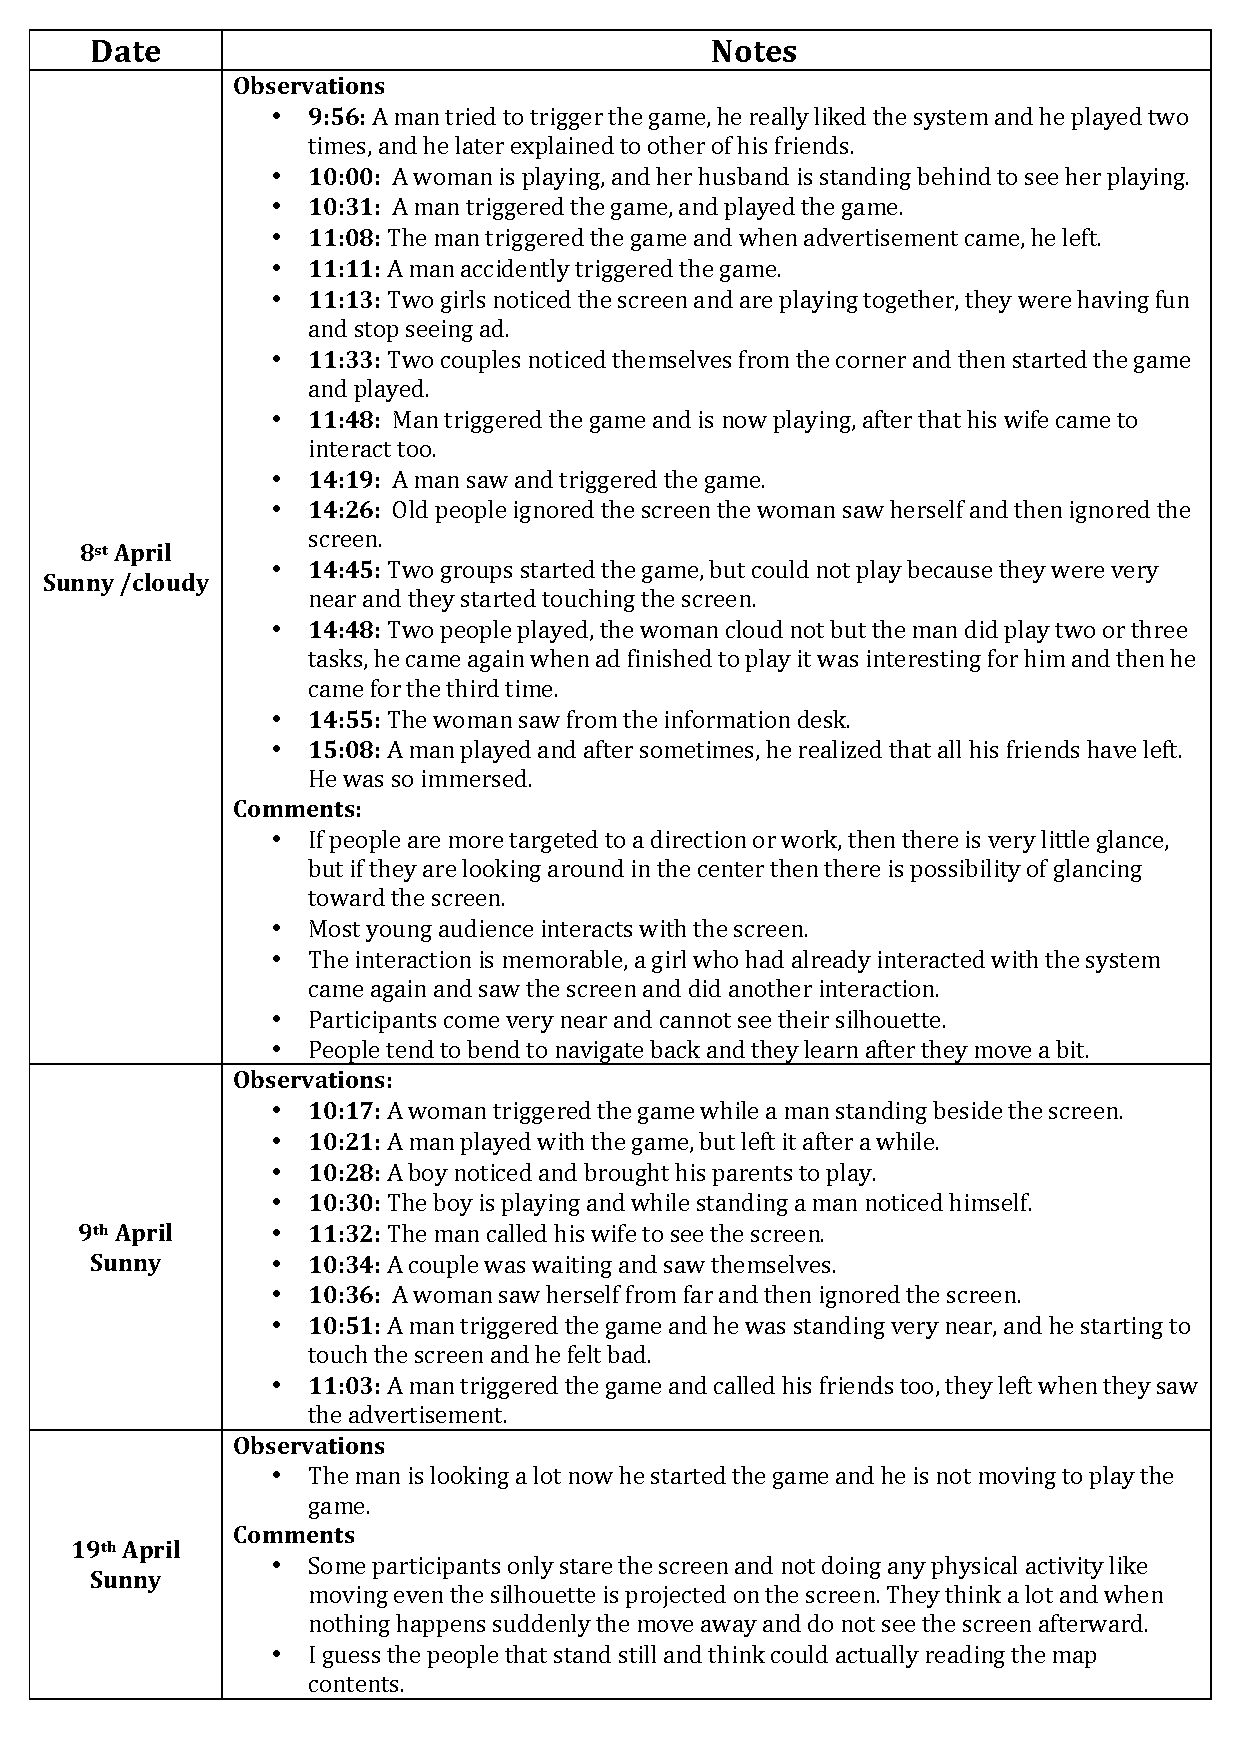
\includegraphics[width=\textwidth,height=0.8\textheight]{Appendices/9/Observation_notes.pdf}
    \caption{Enhanced Interactive observation notes}
     \label{app:EnhancedInteractiveobservationnotes}%
\end{figure}


\chapter{DVD Files and folders}
\setcounter{figure}{0}
\setcounter{table}{0}

\begin{figure}[H]
 \centering 
    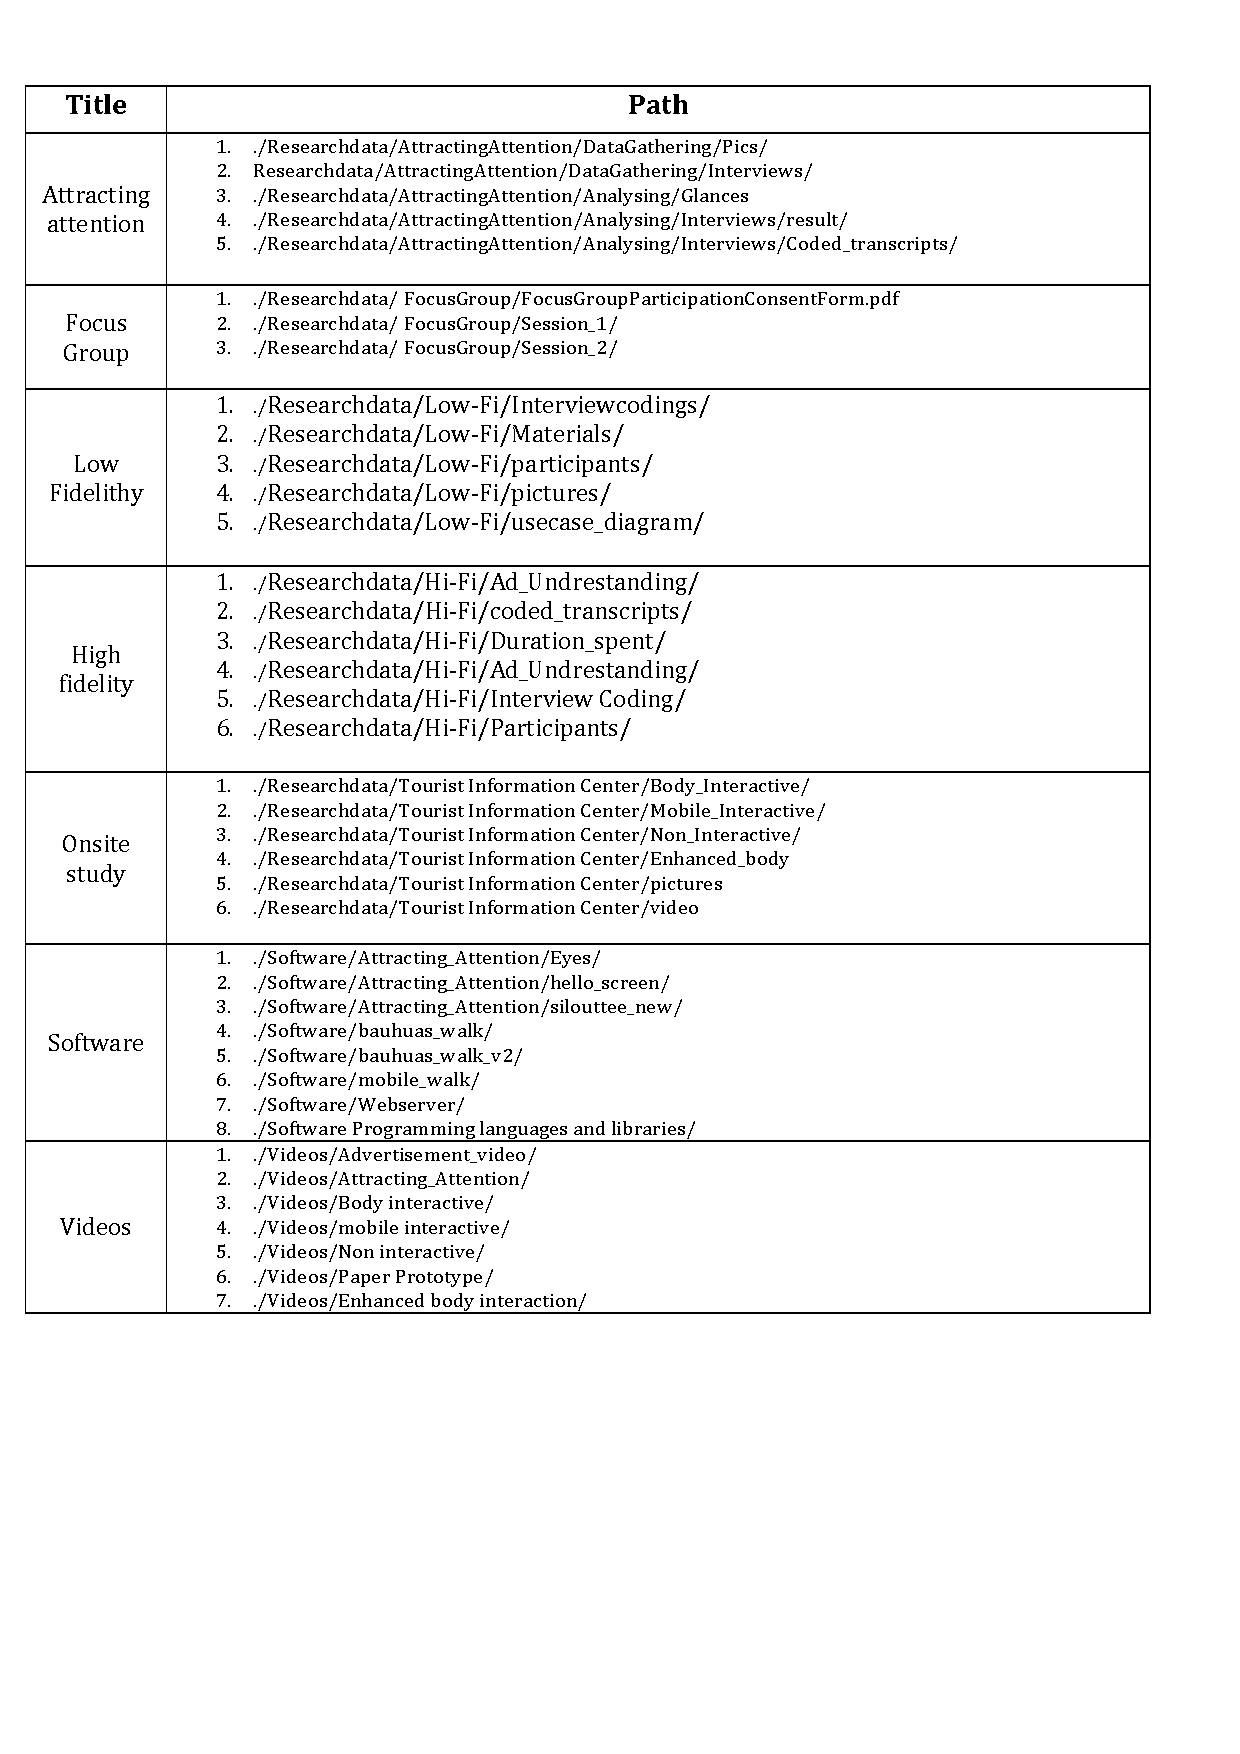
\includegraphics[width=\textwidth,height=0.6\textheight]{Appendices/files_and_folders.pdf}
    \caption{File and Folders in DVD}
     \label{app:fileandfolders}%
\end{figure}



\addtocontents{toc}{\endgroup}
\end{appendices}
